\documentclass{scrreprt}

\usepackage[utf8]{inputenc}
\usepackage[ngerman]{babel}
\usepackage{amsmath}
\usepackage{amsthm}
\usepackage{amssymb}
\usepackage{mathtools}
\usepackage{graphicx}


\newtheorem{defi}{Definition}
\newtheorem{satz}{Satz}

\allowdisplaybreaks
\parskip 12pt

\begin{document}

\tableofcontents

\chapter{Einleitung}
\section{Problembeschreibung}
\label{sec:Problembeschreibung}
Bei synchronen Flow-Shop-Problemen handelt es sich um Produktions\-planungs\-probleme,
bei denen die zu produzierenden Güter (Jobs) z.B. auf einer zyklisch angeordneten Produktionsanlage
produziert werden. Die Produktionsanlage be\-steht aus $m$ Stationen, die sich mit der Anlage drehen.
Außen, um die Anlage herum, befinden sich $m$ fortlaufend nummerierte fixierte Maschinen $M_1,\ldots,M_m$, die die einzelnen Produktionsschritte durchführen.
Dabei handelt es sich bei Maschine $M_1$ um das Einlegen des Jobs in die Anlage und nach der letzten Maschine $M_m$ wird das fertige Produkt entnommen.
Durch Rotation der Anlage werden die Stationen mit den auf ihnen befindlichen Jobs zur jeweils nächsten Maschine transportiert.
Die Reihenfolge, in der alle Jobs die Maschinen durchlaufen müssen ist also fest vorgegeben.
In Abbildung \ref{abb:Anlage} ist eine solche zyklische Anlage dargestellt.
\begin{figure}[h]
    \begin{center}
        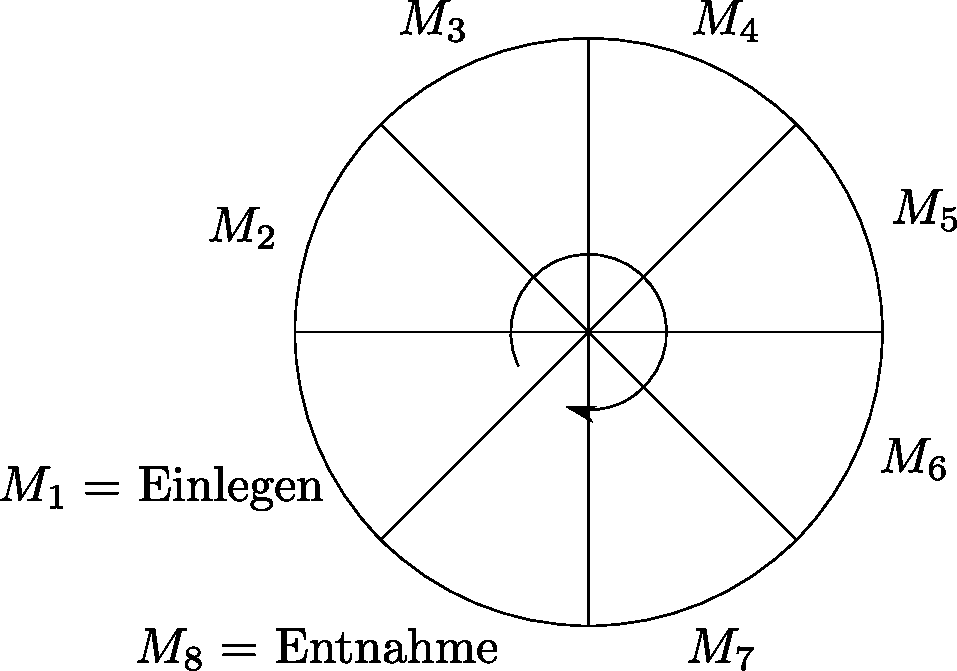
\includegraphics[width=.6\textwidth]{graphics/anlage.pdf}
    \end{center}
    \caption{
        \label{abb:Anlage}
        Kreisförmige Anlage mit $m=8$ Maschinen und Stationen.
    }
\end{figure}
Eine Rotation darf immer nur dann stattfinden, wenn alle Maschinen ihren Produktionsschritt an ihrem aktuellen Job
durchgeführt haben. Auf diese Weise können die Jobs, im Gegensatz zum klassischen (asynchronen) Flow-Shop, 
immer nur \textit{synchron} zur nachfolgenden Maschine gelangen.
Die Zeit, die zwischen zwei Rotationen vergeht, wird als \textit{Zykluszeit} bezeichnet.

Die zu produzierenden Jobs sind gegeben durch die Menge $J=\{1,\ldots,n\}$ 
und die Prozesszeiten von Job $j$ auf Maschine $i$ sind durch $p_{ij}$ gegeben.
Eine Beispielinstanz mit $n=5$ und $m=3$ ist in Tabelle \ref{abb:Bsp} zu sehen.
\begin{figure}[h]
    \begin{center}
        \begin{tabular}{c|ccc}
            & $M_1$ & $M_2$ & $M_3$ \\ \hline
            $1$ & 4 & 6 & 5 \\
            $2$ & 1 & 5 & 6 \\
            $3$ & 2 & 5 & 4 \\
            $4$ & 5 & 2 & 4 \\
            $5$ & 4 & 5 & 4
        \end{tabular}
    \end{center}
    \caption{
        \label{abb:Bsp}
        Beispielinstanz mit 5 Jobs und 3 Maschinen. Die Werte in der Tabelle sind die Prozesszeiten $p_{ij}$.
    }
\end{figure}
\begin{figure}
    \begin{center}
        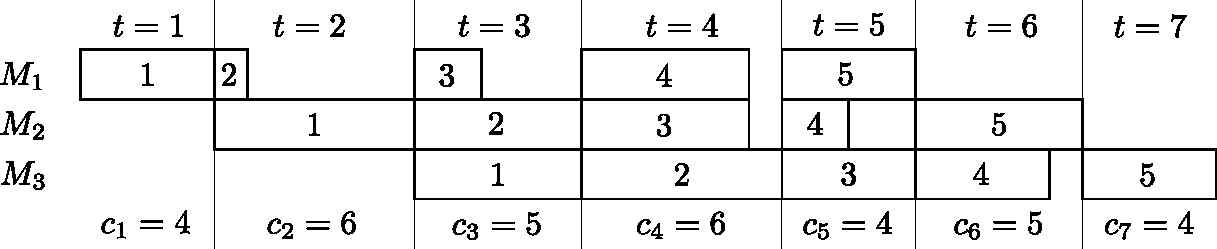
\includegraphics[width=.8\textwidth]{graphics/bspinit.pdf}
    \end{center}
    \begin{center}
        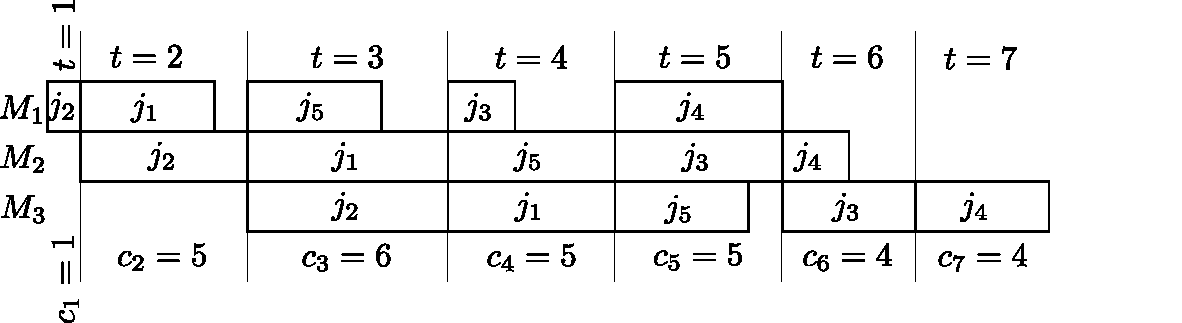
\includegraphics[width=.8\textwidth]{graphics/bspopt.pdf}
    \end{center}
    \caption{
        \label{abb:gantt}
        Gantt-Diagramme der initialen Reihenfolge von Beispiel \ref{abb:Bsp} mit $C_{\max}=34$
        und einer optimalen Reihenfolge mit $C_{\max}=30$.
    }
\end{figure}
Ziel ist es, eine Permutation $\pi$ der Jobs zu erstellen, die die gesamte Produktionsdauer minimiert.
Diese Zielfunktion wird mit $C_{\max}$ bezeichnet.
Die Beispielinstanz \ref{abb:Bsp} ist in Abbildung \ref{abb:gantt} als Gantt-Diagramm aufgetragen.
Oben sind die Jobs in der initialen Reihenfolge und unten in einer bezüglich $C_{\max}$ optimalen Reihenfolge.
Die Zykluszeiten $c_t$ mit $1\leq t\leq n+m-1$ berechnen sich wie folgt:
\[ c_t = \max_{i=\max\{1,t-n+1\}}^{\min\{t,m\}} p_{i\pi_{t-i+1}} \]
Die Zielfunktion lässt sich also durch $C_{\max} = \sum_{t=1}^{n+m-1} c_t$ berechnen.
Andere Zielfunktionen werden in dieser Masterarbeit nicht betrachtet.

Eine Teilmenge $D \subseteq \{1,\ldots,m\}$ der Maschinen heißt \textit{dominierend}, wenn 
\[ p_{dj} \geq p_{ej} \quad \forall j\in J, d\in D, e\not\in D \] 
ist. Die Prozesszeiten aller Jobs auf dominierenden Maschinen sind also immer mindestens so groß wie die Prozesszeiten auf den restlichen Maschinen.
Treten dominierende Maschinen auf, müssen für die Berechnung der Zykluszeiten die Prozesszeiten auf den übrigen Maschinen also nicht betrachtet werden.

Zusätzlich benötigen die Jobs unter Umständen Ressourcen aus einer Menge $R$, um in die Stationen eingelegt werden zu können. Diese Ressourcen können erst nach
Fertigstellung eines Jobs, also nachdem er nach Maschine $M_m$ aus der Anlage genommen wurde, wiederverwendet werden.
Sie sind allerdings nur in begrenzter Zahl vorhanden und im Allgemeinen ist nicht jede Ressource für jeden Job geeignet.
Für $j\in J$ sei $\rho_j\subseteq R$ die Menge der Ressourcen, die für $j$ geeignet ist.
Umgekehrt sei für $r\in R$ mit $\iota_r\subseteq J$ die Menge der Jobs bezeichnet, für die $r$ geeignet ist.
An Maschine $M_1$ kann es daher notwendig sein, vor dem Einlegen des nächsten Jobs die Ressource zu wechseln, 
wenn auf der entsprechenden Station zuvor Job $j\in J$ mit Ressource $r\in\rho_j$ fertiggestellt wurde 
und nun Job $j'\not\in\iota_r$ eingelegt werden soll.

Für die Ressourcen können folgende Situationen auftreten:
\begin{itemize}
    \item Alle Ressourcen sind für alle Jobs geeignet, also $\rho_j=R$ für alle $j\in J$.
    \item Die Jobs lassen sich in disjunkte Gruppen unterteilen, so dass für alle Jobs aus einer Gruppe dieselbe Ressourcenmenge geeignet ist.
        Wenn also $\rho_i \cap \rho_j \neq \emptyset$, dann folgt $\rho_i=\rho_j$.
    \item Die Ressourcenmengen bilden Hierarchien. 
        D.h., wenn $\iota_q \cap \iota_r \neq \emptyset$, dann folgt $\iota_q \subseteq \iota_r$ oder $\iota_r \subseteq \iota_q$.
    \item Die $\rho_j$ sind beliebige Teilmengen von $R$.
\end{itemize}%
Neben dem Wechsel von Ressourcen, der zusätzliche Zeit in Anspruch nimmt, können auch andere Formen von \textit{Rüstkosten}
auftreten. Z.B. kann es sein, dass an einer Station zunächst einige Umstellungen vorgenommen werden müssen, bevor der
neue Job eingelegt werden kann. Die Jobs können in Familien $\mathcal{F}$ eingeteilt werden, so dass beim Übergang
zwischen zwei Jobs aus den Familien $f$ und $g$ die Rüstkosten $s_{fg}$ auftreten.
Diese Rüstkosten können 
\begin{itemize}
    \item sowohl vom Vorgänger als auch vom Nachfolger abhängig sein ($s_{fg}$), 
    \item nur vom Nachfolger abhängig sein ($s_{fg} = s_{g}$) oder
    \item konstant sein ($s_{fg} = s > 0$).
\end{itemize}%
Dabei wird $s_{ff} = 0$ angenommen für alle $f\in\mathcal{F}$, dass also keine Rüstkosten innerhalb einer Familie auftreten.
Wenn Ressourcen notwendig sind, können die Familien über die Ressourcen definiert werden:
Wenn $\rho_i=\rho_j$, dann gehören $i$ und $j$ zur gleichen Familie.
Das setzt allerdings voraus, dass für $i$ und $j$ auf jeden Fall die selbe Ressource verwendet wird, falls sie in $\pi$ im Abstand von $m$ vorkommen.

Wenn Rüstkosten auftreten, soll nicht mehr nur die Summe aller Zykluszeiten minimiert werden, sondern zusätzlich noch die Summe aller auftretenden Rüstkosten.
Diese Zielfunktion lässt sich als 
\[ \min\left(C_{\max}+\sum_{i=1}^{n-m}s_{i,i+m}\right) \] 
formulieren, wobei hier die Rüstkosten direkt mit den Jobs statt mit den Familien indiziert sind.

\begin{figure}
    \begin{center}
        \begin{tabular}{c|ccccc}
            & $j_1$ & $j_2$ & $j_3$ & $j_4$ & $j_5$ \\ \hline
            $1$ & 0 & 8 & 5 & 9 & 4\\
            $2$ & 6 & 0 & 6 & 8 & 8\\
            $3$ & 4 & 7 & 0 & 5 & 4\\
            $4$ & 5 & 7 & 8 & 0 & 9\\
            $5$ & 4 & 5 & 8 & 9 & 0
        \end{tabular}
    \end{center}
    \caption{
        \label{abb:BspRes}
        Rüstkosten für die Beispielinstanz aus Tabelle \ref{abb:Bsp}.
        Beispielsweise treten Rüstkosten von $6$ auf, wenn von $j_2$ auf $j_1$ gewechselt werden muss.
    }
\end{figure}
In Abbildung \ref{abb:BspRes} ist eine mögliche Rüstkostentabelle für das Beispiel aus \ref{abb:Bsp} gegeben.
Die initiale Reihenfolge und eine optimale sind in Abbildung \ref{abb:ganttres} als Gantt-Diagramm dargestellt.
\begin{figure}
    \begin{center}
        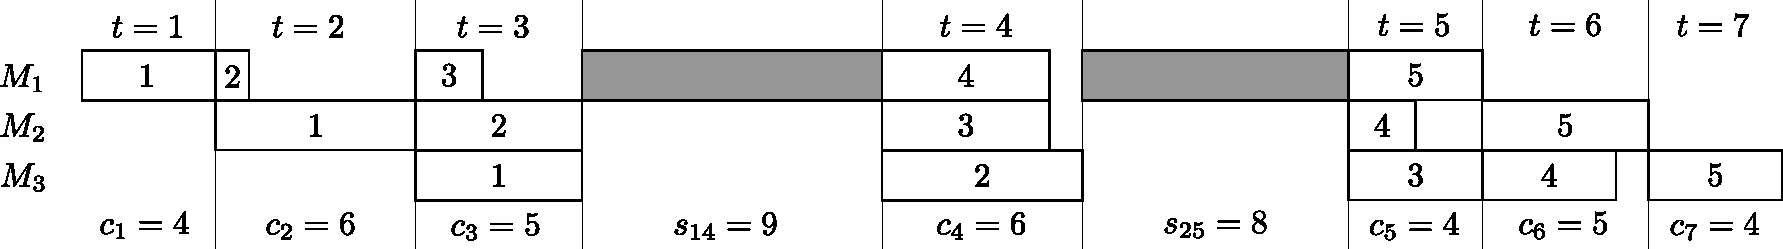
\includegraphics[width=\textwidth]{graphics/bspresinit.pdf}
    \end{center}
    \begin{center}
        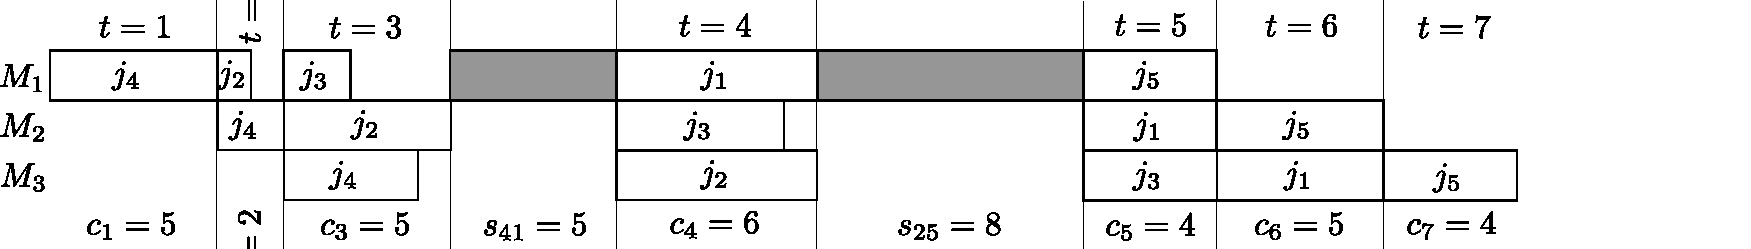
\includegraphics[width=\textwidth]{graphics/bspresopt.pdf}
    \end{center}
    \caption{
        \label{abb:ganttres}
        Initiale und eine optimale Lösung als Gantt-Diagramme für das Beispiel aus \ref{abb:Bsp} erweitert um Rüstkosten aus \ref{abb:BspRes}.
    }
\end{figure}

Insgesamt gilt es, neben der Reihenfolge $\pi$ auch ein Mapping $f:J\rightarrow R$ zu finden, 
das jedem Job $j\in J$ eine Ressource $r\in\rho_j$ zuweist und folgenden Ansprüchen genügt:
\begin{itemize}
    \item $f$ muss zulässig sein in dem Sinne, dass beim Einlegen jedes Jobs $j\in J$ eine Ressource $r\in\rho_j$ verfügbar ist
        (d.h., dass $r$ sich nicht gerade an anderer Stelle in der Anlage befindet).
    \item $f$ und $\pi$ zusammen sollen optimal sein in dem Sinne, dass die Summe aus den durch $\pi$ und $f$ definierten Zykluszeiten und 
        Rüstkosten minimal ist.
\end{itemize}

Im Folgenden wird ein Mixed Integer Linear Program (MIP) vorgestellt, dass das Gesamtproblem löst, allerdings ohne die Verfügbarkeit von Ressourcen zu beachten:
\begin{align}
    \text{min} \quad \sum_{t=1}^{n+m-1} &c_t + \sum_{j=1}^n \sum_{h=1}^n s_{jh} y_{jh} \label{allmip:obj}\\
    \text{s.t.}\quad \sum_{k=1}^n x_{jk} &= 1 & j\in N \label{allmip:1}\\
                     \sum_{j=1}^n x_{jk} &= 1 & k\in N \label{allmip:2}\\
    c_t &\geq \sum_{j=1}^n p_{t-k+1,j} \cdot x_{jk} & t\in T, k=\max\{1,t-m+1\},\ldots,\min\{n,t\} \label{allmip:3}\\
    y_{jh} + 1 &\geq x_{j,k-m} + x_{hk} & j,h\in N, k=m+1,\ldots,n \label{allmip:4}\\
    c_t &\geq 0 & t\in T \\
    x_{jk} &\in \{0,1\} & j,k\in N \\
    y_{jh} &\in \{0,1\} & j,h\in N
\end{align}
$N$ ist die Indexmenge der Jobs, also $N=\{1,\ldots,n\}$ und $T=\{1,\ldots,n+m-1\}$ ist die Indexmenge der Zykluszeiten.
Die Binärvariablen $x_{jk}$ geben an, an welcher Position $k$
sich Job $j$ befindet. Es gilt $x_{jk}=1$ genau dann, wenn $j$ an
Position $k$ ist. Die Nebenbedingungen \ref{allmip:1} und \ref{allmip:2}
stellen sicher, dass sich jeder Job an genau einer Position befindet und 
dass sich an jeder Position genau ein Job befindet.
In Nebenbedingung \ref{allmip:3} werden die Zykluszeiten bestimmt.
Den Binärvariablen $y_{jh}$ wird in Nebenbedingung \ref{allmip:4} folgende
Bedeutung gegeben: $y_{jh}=1$, wenn Job $j$ genau $m$ Positionen
vor Job $h$ in $\pi$ liegt.
In der Zielfunktion \ref{allmip:obj} wird dann die Summe aus allen
Zykluszeiten gebildet und die Summe aller Rüstkosten $s_{jh}$, die beim
Übergang von Job $j$ zu $h$ auftreten.

Obwohl in diesem MIP nicht die Verfügbarkeiten von Ressourcen beachtet werden,
benötigt es schon bei $n=20$ mehrere Stunden zum Finden der optimalen Lösung.
Es ist also für Instanzen mit mehreren Tausend Jobs nicht geeignet.
Aufgrund dieser Tatsache ist eine heuristische Herangehensweise an 
synchrone Flow-Shop-Probleme mit Ressourcen und Rüstkosten eine gute Alternative.


\section{Motivation für Dekompositionsansätze}
In \cite{...} wurde gezeigt, dass schon das Optimieren bezüglich $C_{\max}$, also ohne Ressourcen und Rüstkosten, $\mathcal{NP}$-schwer ist für $m>2$.
Versuche, dieses Problem -- oder auch einige Spezialfälle davon -- mit ganzzahliger linearer Programmierung optimal zu lösen, waren nur für sehr kleine Instanzen mit
$n<30$ in hinnehmbarer Zeit erfolgreich, was weit hinter praktischen Anforderungen zurückliegt (vgl. Abschnitt \ref{subsec:LineareProgrammierung}).
Aufgrund der Komplexität des Gesamtproblems (vgl. das MIP aus Abschnitt \ref{sec:Problembeschreibung} sollen in dieser Arbeit zwei Dekompositionsansätze verfolgt werden:
\begin{enumerate}
    \item Zunächst wird eine Reihenfolge $\pi$ aufgestellt, ohne Ressourcen und Rüstkosten zu betrachten, so dass $C_{\max}$ möglichst gut ist.
        Anschließend wird ein Mapping $f$ basierend auf $\pi$ erstellt, möglichst ohne nachträgliche Änderung an $\pi$ vorzunehmen.
    \item Es wird zuerst ein Mapping $f$ erstellt, so dass die Ressourcen zulässig zugewiesen sind und die durch die Ressourcenwechsel verursachten Rüstkosten minimal sind.
        Anschließend werden, ohne $f$ zu verändern, die Jobs so in einer Reihenfolge $\pi$ angeordnet, dass die Zykluszeiten möglichst minimal sind.
\end{enumerate}%
Beide Ansätze liefern natürlich im Allgemeinen keine optimalen Lösungen, da jeweils getrennt bezüglich $\pi$ und $f$ optimiert wird,
obwohl die optimale Lösung von beiden zusammen abhängig ist.
Außerdem sind selbst die aus den Ansätzen resultierenden Teilprobleme teilweise noch $\mathcal{NP}$-schwer.
Beispielsweise ist bei Ansatz (1) das Berechnen einer $C_{\max}$-optimalen Reihenfolge $\pi$ in dem Spezialfall,
dass es nur eine dominierende Maschine gibt trivial, da $C_{\max}$ bei jeder Reihenfolge identisch ist,
und wenn es genau zwei benachbarte dominierende Maschinen gibt,
ist es mit dem Algorithmus von Gilmore und Gomory \cite{...} in Polynomialzeit lösbar.
Bei der anschließenden Zuweisung von Ressourcen ist noch unbekannt, ob ein polynomieller Algorithmus existiert.
%Dies herauszufinden ist eines der Ziele dieser Arbeit.

Je nachdem, ob die Rüstkosten die Zykluszeiten dominieren oder umgekehrt, ist Ansatz (2) bzw. Ansatz (1) vielversprechender.


\chapter{Der erste Dekompositionsansatz}
Beim ersten Dekompositionsansatz wird zunächst eine (möglichst gute) Jobreihenfolge $\pi$ bestimmt.
Dabei werden Ressourcen und Rüstkosten außer Acht gelassen. 
Es wird also zunächst ausschließlich $C_{\max}$ optimiert. Anschließend wird ein Mapping $f$ aufgestellt,
so dass Ressourcen nur dann eingeplant werden, wenn sie auch zur Verfügung stehen, und darüber hinaus
möglichst selten ausgetauscht werden müssen, so dass geringe Rüstkosten auftreten.

In Abschnitt \ref{sec:BerechnenEinerJobreihenfolge} werden einige exakte und heuristische Verfahren für die
Berechnung einer $C_{\max}$-optimalen Reihenfolge $\pi$ vorgestellt, was im Allgemeinen $\mathcal{NP}$-schwer ist.
Anschließend werden in Abschnitt \ref{sec:ZuweisungVonRessourcen} Verfahren vorgestellt, die ein möglichst gutes Mapping $f$ erzeugen.
Dabei wird speziell darauf eingegangen, ob mit der gegebenen Reihenfolge $\pi$ und den gegebenen Ressourcen
überhaupt eine zulässige Lösung möglich ist, und, wie dann ggf. die Zulässigkeit durch nachträgliche Änderungen an $\pi$
erzeugt werden kann.

\section{Berechnen einer Jobreihenfolge}
\label{sec:BerechnenEinerJobreihenfolge}
Das Finden einer $C_{\max}$-optimalen Jobreihenfolge ist im Allgemeinen $\mathcal{NP}$-schwer.
Daher wird im ersten Unterabschnitt \ref{subsec:LineareProgrammierung} zunächst ein MIP vorgestellt,
das solch eine Reihenfolge findet.
Anschließend wird in Unterabschnitt \ref{subsec:DerAlgorithmusVonGilmoreUndGomory} auf einen Spezialfall eingegangen, der in polynomieller Zeit lösbar ist.
Danach werden in \ref{subsec:HeuristischeVerfahren} einige heuristische Verfahren vorgestellt.

\subsection{Ganzzahlige Lineare Programmierung}
\label{subsec:LineareProgrammierung}
Zum Finden einer $C_{\max}$-optimalen Lösung wurde folgendes MIP aufgestellt, das in dieser Form auch schon in \cite{...} vorgestellt wurde.
Es ist identisch mit dem MIP in Abschnitt \ref{sec:Problembeschreibung} bis auf die Nichtberücksichtigung der Rüstkosten.
\begin{align}
    \text{min} \quad \sum_{t=1}^{n+m-1} &c_t \\
    \text{s.t.}\quad \sum_{k=1}^n x_{jk} &= 1 & j\in N \\
                     \sum_{j=1}^n x_{jk} &= 1 & k\in N \\
    c_t &\geq \sum_{j=1}^n p_{t-k+1,j} \cdot x_{jk} & t\in T, k=\max\{1,t-m+1\},\ldots,\min\{n,t\} \\
    c_t &\geq 0 & t\in T \\
    x_{jk} &\in \{0,1\} & j,k\in N
\end{align}
Dieses MIP liefert für Instanzen mit $n\leq 30$ eine optimale Lösung in unter einer Stunde.
Diese Laufzeiten sind zwar schon deutlich besser als die Variante mit Rüstkosten in Abschnitt \ref{sec:Problembeschreibung},
bei größeren Instanzen ist dieser Zeitaufwand allerdings immer noch nicht praktikabel. 

Für Instanzen mit $n\leq 500$ ist die beste nach einer halben Stunde gefundene Lösung (obere Schranke) in ihrer Güte vergleichbar mit den Heuristiken,
die in Unterabschnitt \ref{subsec:HeuristischeVerfahren} vorgestellt werden (für einen Vergleich s. \ref{subsec:VergleichDerHeuristiken}).
In diesem Sinne kann dieses MIP daher ebenfalls als Heuristik betrachtet werden.


\subsection{Der Algorithmus von Gilmore und Gomory}
\label{subsec:DerAlgorithmusVonGilmoreUndGomory}
Der Algorithmus von Gilmore und Gomory \cite{...} löst in $\mathcal{O}(n\log n)$ einen speziellen Fall des gerichteten Travelling-Salesman-Problems (TSP),
bei dem alle Knoten $i$ zwei Parameter $a_i,b_i$ haben und die Kantenkosten $c_{ij}$ zwischen je zwei Knoten $i$ und $j$ nur von $a_i$ und $b_j$ abhängig sind.

Diese Situation liegt beim synchronen Flow-Shop vor, wenn es nur zwei benachbarte dominierende Maschinen gibt.
O.B.d.A seien dies $M_1$ und $M_2$.
Jobs können durch Knoten repräsentiert werden und die beiden Prozesszeiten auf den dominierenden Maschinen liefern die Parameter $a_i$ und $b_i$. 
Der Abstand zwischen zwei Knoten entspricht dann der Zykluszeit, die die entsprechenden Jobs verursachen, wenn sie nebeneinander liegen.
Die Berechnung der Zykluszeiten vereinfacht sich hier zu
$c_t = \max \{p_{2\pi_{t-1}},p_{1\pi_t}\}$ für $2\leq t\leq n$.
Sie sind also für je zwei Jobs $\pi_{t-1},\pi_{t}$ nur noch von der Prozesszeit des vorderen Jobs auf der zweiten Maschine ($p_{2\pi_{t-1}}$) 
und der Prozesszeit des hinteren Jobs auf der ersten Maschine ($p_{1\pi_t}$) abhängig.

Auf die Funktionsweise des Algorithmus soll in dieser Arbeit nicht näher eingegangen werden.
Eine Anwendung des Algorithmus von Gilmore und Gomory als Heuristik für ein Problem mit mehreren dominierenden Maschinen wird in
\ref{subsubsec:ggHeuristik} beschrieben.


\subsection{Heuristische Verfahren}
\label{subsec:HeuristischeVerfahren}
Aufgrund der $\mathcal{NP}$-Schwere der Optimierung von $C_{\max}$ im allgemeinen Fall und der schlechten Laufzeit des MIPs aus Abschnitt \ref{subsec:LineareProgrammierung}
bei Instanzen realer Größe werden hier einige heuristische Ansätze zur Berechnung von $\pi$ vorgestellt.

\subsubsection{Non-Full-Schedule-Heuristik}
Diese Heuristik ist eine konstruktive Greedy-Heuristik, die Schritt für Schritt einen Job an $\pi$ anhängt, beginnend mit einer leeren Reihenfolge.
Sie arbeitet ähnlich wie die Nearest-Neighbor-Heuristik beim TSP.
In jeder Iteration werden alle noch verbleibenden Jobs bewertet und der Job mit der besten Bewertung wird an $\pi$ angehängt.
Die Heuristik benötigt also genau $n$ Iterationen.
Die Bewertungsfunktion betrachtet die letzten $m-1$ Zykluszeiten der noch nicht fertigen Reihenfolge, 
wobei die Zykluszeiten am Anfang bei einer noch leeren Reihenfolge als $0$ angenommen werden.
Für jeden Job $j$, der noch nicht in $\pi$ ist, werden diese $m-1$ Zykluszeiten mit den ersten $m-1$ Prozesszeiten von $j$ verglichen.
Die Idee ist, dass diese möglichst übereinstimmen sollten. Ist eine Prozesszeit sehr viel größer als die aktuelle Zykluszeit,
zu der sie hinzugefügt werden würde, würde die Zykluszeit entsprechend um einen Wert $c_+$ ansteigen.
Ist umgekehrt die Zykluszeit sehr viel größer als die zugehörige Prozesszeit von $j$, dann würde diese kurze Prozesszeit verschenkt werden.
Die Differenz aus Zykluszeit und Prozesszeit wird mit $c_-$ bezeichnet.
Die Bewertungsfunktion berechnet für jeden Job die Summe aus den $m-1$ $c_+$-Werten.
Diese Summe ist die Bewertung für einen Job $j$. Der Job mit der kleinsten Bewertung wird an $\pi$ angehängt.
Falls mehrere Jobs eine optimale Bewertung haben, wird für diese Jobs als zweites Kriterium die Summe der $c_-$-Werte betrachtet.
Der Job, bei dem diese Summe am kleinsten ist, verschenkt am wenigsten Zeit und wird ausgewählt.
Das Vorgehen dieser Heuristik wird anhand der Beispielinstanz \ref{abb:Bsp} in Abbildung \ref{abb:nfsbsp} veranschaulicht.
\begin{figure}
    \begin{center}
%        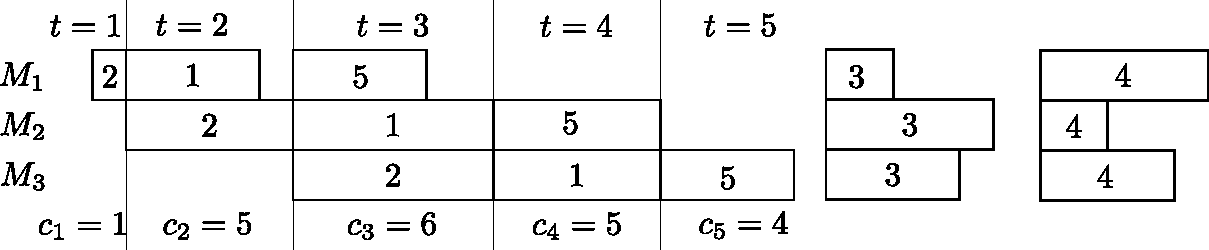
\includegraphics[width=.8\textwidth]{nfsbsp.pdf}
    \end{center}
    \caption{
        \label{abb:nfsbsp}
    }
\end{figure}

Da in jeder Iteration alle verbleibenden Jobs betrachtet werden und für jeden dieser Jobs $m-1$ Zeiten verglichen werden,
liegt die asymptotische Laufzeit dieser Heuristik in $\mathcal{O}(n^2m)$.

\subsubsection{Double Ended Non-Full-Schedule-Heuristik}
Diese Heuristik basiert auf der Non-Full-Schedule-Heuristik.
Der Unterschied besteht darin, dass $\pi$ nicht nur von vorne, sondern gleichzeitig auch von hinten zur Mitte hin aufgebaut wird.
Jeder noch nicht in $\pi$ enthaltene Job wird pro Iteration mit beiden Enden der bisherigen Reihenfolge verglichen.
Die Bewertungsfunktion für das hintere Ende arbeitet analog.
Es wird der beste Job für das vordere Ende und der beste für das hintere Ende gesucht und der mit der besseren Bewertung wird vorne bzw. hinten eingefügt.
Die asymptotische Laufzeit liegt hier ebenfalls in $\mathcal{O}(n^2m)$.

\subsubsection{Gilmore-Gomory-Heuristik}
\label{subsubsec:ggHeuristik}
Diese Heuristik wendet den Algorithmus von Gilmore und Gomory auf beliebige Instanzen an.
Es können zwei Fälle eintreten:
\begin{enumerate}
    \item Unter den dominierenden Maschinen $D$ gibt es zwei, die benachbart sind, also $\exists i\in\{1,\ldots,m\}$ mit $i,i+1\in D$.
    \item Es gibt keine benachbarten dominierenden Maschinen.
\end{enumerate}
Wenn Fall (2) eintritt, werden alle $m$ Maschinen als dominierend angesehen, da dies für den Algorithmus keine Einschränkung darstellt.
Nun werden zwei benachbarte dominierende Maschinen gewählt.
O.B.d.A seien dies die Maschinen $M_1$ und $M_2$. Seien 
\begin{align} 
    d_{\min} &\coloneqq \min_{\substack{i\in \{1,2\} \\ j\in J}} p_{ij} \\
    e_{\max} &\coloneqq \max_{\substack{i\not\in \{1,2\} \\ j\in J}} p_{ij} \\
    K &\coloneqq \frac{e_{\max}}{d_{\min}} \text{,}
\end{align}
wobei $d_{\min}=0$ und daraus folgend $K=\infty$ erlaubt sind. 
Nun wird aus der gegebenen Instanz $I$ eine neue Instanz $I'$ erzeugt, die sich nur dadurch von $I$ unterscheidet, dass die Prozesszeiten
auf allen dominierenden Maschinen außer auf $M_1$ und $M_2$ mit $\frac{1}{K}$ skaliert werden, also
\begin{align}
    p'_{ij} \coloneqq \begin{cases} \frac{p_{ij}}{K} &\text{für } i\in D\setminus\{1,2\} \\ p_{ij} &\text{sonst.} \end{cases}
\end{align}
Auf diese Weise sind $M_1$ und $M_2$ in $I'$ die einzigen dominierenden Maschinen und folglich kann $I'$ mit dem Algorithmus von Gilmore und Gomory optimal gelöst werden.
Die resultierende Reihenfolge $\pi$ wird als heuristische Lösung für die ursprüngliche Instanz $I$ verwendet.

Da die Prozesszeiten der in $I'$ vernachlässigten dominierenden Maschinen sich um den Faktor $K$ von denen in $I$ unterscheiden, 
können sich die aus $\pi$ ergebenen Zykluszeiten von $I$ und $I'$ auch maximal um den Faktor $K$ unterscheiden:
\begin{align}
    c_t \leq K\cdot c'_t \quad \forall 1\leq t\leq n+m-1
\end{align}
Da die optimale Lösung von $I'$ eine untere Schranke für die optimale Lösung von $I$ ist, also $C'_{\max} \leq C_{\max}$, folgt für die Lösung $L_{GG}$ der
Gilmore-Gomory-Heuristik:
\begin{align}
    L_{GG} \leq K\cdot C'_{\max} \leq K\cdot C_{\max}
\end{align}
Die Gilmore-Gomory-Heuristik hat also eine relative Gütegarantie von $K$.
Bei der Wahl der beiden benachbarten dominierenden Maschinen sollte darauf geachtet werden, dass $d_{\min}$ möglichst groß und $e_{\max}$ möglichst klein ist.
Dadurch ist dann auch der Gütefaktor $K$ am kleinsten.

Das Finden der geeigneten dominierenden Maschinen kann in $\mathcal{O}(nm)$ durchgeführt werden. 
Das Anpassen der Prozesszeiten der übrigen dominierenden Maschinen ist nur in der Theorie von Interesse.
Der Gilmore-Gomory-Algorithmus kann diese einfach ignorieren.
Die Gesamtlaufzeit beträgt daher $\mathcal{O}(nm + n\log n)$.

Für die weitere Analyse dieser Heuristik soll der Begriff der \textit{Semidominanz} eingeführt werden.
Die Semidominanz ist ein Maß dafür, wie weit eine Teilmenge von Maschinen davon entfernt ist, dominierend zu sein.
Eine Semidominanz von $0$ bedeutet, die Maschinen sind dominierend.
Für eine Teilmenge von Maschinen $D\subseteq\{1,\ldots,m\}$ sei 
\[d_{\min} = \min_{\substack{i\in D \\ j\in\{1,\ldots,n\}}} p_{ij}\] 
die kleinste ihrer Prozesszeiten, analog zur obigen Definition von $d_{\min}$.
Die Semidominanz ist dann definiert als
\[\mathcal{D}_{D} \coloneqq \sum_{i\not\in D} \sum_{j=1}^n \max\{0,p_{ij}-d_{\min}\} \text{.}\]
Unabhängig von der \textit{relativen} Gütegarantie $K$ liefert diese Heuristik auch eine \textit{absolute} Gütegarantie von $\mathcal{D}_{\{i,i+1\}}$, 
wenn $M_i$ und $M_{i+1}$ als benachbarte Maschinen ausgewählt werden.
Die Gilmore-Gomory-Heuristik liefert also besonders gute Näherungen, wenn zwei benachbarte Maschinen fast dominierend sind und nur wenige Prozesszeiten auf anderen
Maschinen dies verhindern.

\subsubsection{Nachbarschaftssuche}
\label{subsubsec:Nachbarschaftssuche}
Mit einer Nachbarschaftssuche können bereits existierende (nicht optimale) Reihenfolgen verbessert werden.
Mögliche Nachbarschaftsoperatoren sind
\begin{itemize}
    \item $\mathit{xch}_{jk}$: vertauscht die Jobs an den Positionen $j$ und $k$ miteinander,
    \item $\mathit{shift}_{jk}$: "`shiftet"' den Job an Position $j$ nach Position $k$. 
        Alle Jobs zwischen $j$ und $k$ rücken um eins nach links (falls $j<k$) bzw. nach rechts (falls $j>k$).
\end{itemize}
Auf Grundlage dieser Nachbarschaften lassen sich außerdem z.B. Iterative Improvement, eine Tabu-Suche oder Simulated Annealing implementieren.

Im Rahmen dieser Arbeit wurde ein Simulated Annealing Algorithmus auf Grundlage der $\mathit{xch}_{jk}$-Nachbarschaft implementiert.
Es wird mit einer zufälligen initialen Reihenfolge $\pi$ begonnen.
Die Funktion, die $C_{\max}$ von $\pi$ berechnet, sei mit $c$ bezeichnet.
Pro Iteration werden zufällige $j$ und $k$ bestimmt, mit denen eine benachbarte Lösung $\pi' = \mathit{xch}_{jk}(\pi)$ erzeugt wird.
Ist $\pi'$ besser als die aktuelle Lösung $\pi$, d.h. $c(\pi') < c(\pi)$, wird $\pi'$ als neue Lösung übernommen.
Ist $\pi'$ schlechter als $\pi$, wird $\pi'$ nur mit einer bestimmten Wahrscheinlichkeit übernommen.
Diese Wahrscheinlichkeit beträgt $e^{\frac{c(\pi)-c(\pi')}{t_i}}$, wobei $(t_i)_i$ eine Nullfolge ist 
und $i$ die Anzahl der bisher durchgeführten Iterationen angibt.
Die Folge $(t_i)_i$ wird auch als "`Temperatur"' bezeichnet, die im Laufe des Verfahrens abnimmt.
Es wurde mit unterschiedlichen Temperaturen experimentiert.
Es wurden 
\begin{itemize}
    \item $t_i = \alpha t_{i-1}$ für unterschiedliche $\alpha\in]0,1[$ und 
    \item $t_i = \frac{c}{i}$, 
    \item $t_i = \frac{c}{\log i}$ und 
    \item $t_i = c \frac{|\cos\frac{i}{30}|}{i}$
\end{itemize}
jeweils für unterschiedliche $c\in\mathbb{R}_+$ getestet. Die besten Resultate lieferte $t_i = 50\frac{|\cos\frac{i}{30}|}{i}$.
Durch den Cosinus schwankt die Temperatur, so dass abwechselnd verschlechternde Lösungen erlaubt bzw. nicht erlaubt werden.
Das Verfahren terminiert, sobald in 1000 aufeinander folgenden Iterationen keine neue beste Lösung gefunden werden konnte.

Dieser Simulated Annealing Algorithmus lieferte in Tests meist etwas bessere Ergebnisse als die übrigen Heuristiken.
Die Heuristiken werden im nachfolgenden Unterabschnitt \ref{subsec:VergleichDerHeuristiken} evaluiert.


\subsection{Vergleich der Heuristiken}
\label{subsec:VergleichDerHeuristiken}
In diesem Abschnitt werden die Rechenergebnisse der Heuristiken aus Unterabschnitt \ref{subsec:HeuristischeVerfahren} vorgestellt und miteinander verglichen.
Es wurden drei Testreihen mit zufälligen Instanzen erzeugt, jeweils mit $m=8$ und $n=50,100,150,\ldots,5000$.
Getestet wurde auf einem PC mit Intel(R) Xeon(R) CPU E3-1230 v3, 8 Kerne @ 3.30GHz, und 16GB RAM unter Ubuntu 13.10.
Die MIPs wurden mit ZIMPL \cite{Koch2004} und CPLEX v12.6 gelöst.
Die übrigen Heuristiken wurden in C++ implementiert und mit dem GCC v4.8.1 mit O2-Optimierung kompiliert.

In der ersten Testreihe sind die Maschinen $M_3,M_4,M_5$ dominierend.
Ihre Prozesszeiten wurden gleichverteilt aus dem Intervall $[10,100]$ gewählt.
Die Prozesszeiten der übrigen Maschinen wurden aus dem Intervall $[0,9]$ gleichverteilt gewählt.
In Abbildung \ref{abb:3dom} sind die Resultate aufgetragen.
\begin{figure}
    \begin{center}
        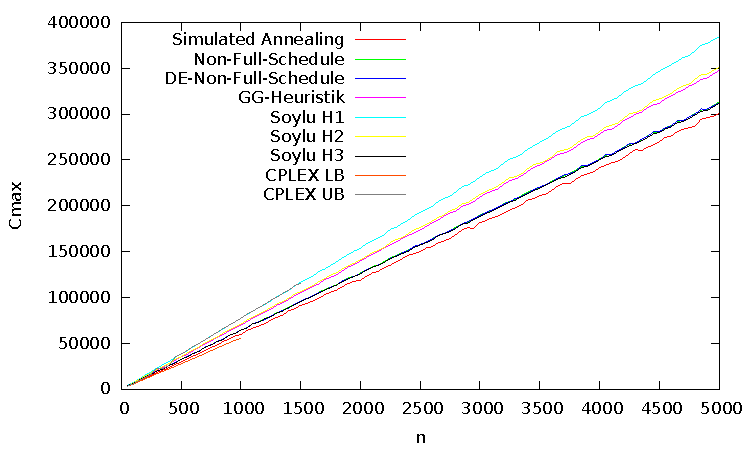
\includegraphics[width=.8\textwidth]{../instances/3dom/plot.pdf}
    \end{center}
    \begin{center}
        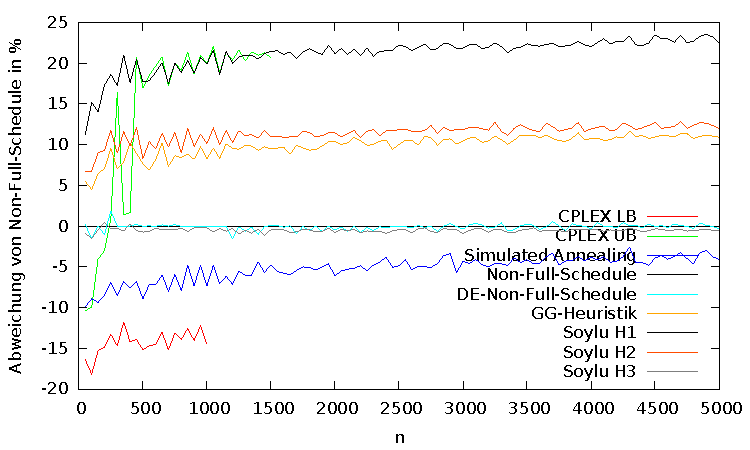
\includegraphics[width=.8\textwidth]{../instances/3dom/plotrel.pdf}
    \end{center}
    \caption{
        \label{abb:3dom}
        Absolute (oben) und relative (unten) Unterschiede zwischen der Non-Full-Schedule-Heuristik und den übrigen Heuristiken
        bei drei dominierenden Maschinen (gleichverteilte Prozesszeiten).
    }
\end{figure}
Aufgetragen sind jeweils die absoluten Differenzen $C_{\max,h}-C_{\max,nfs}$ der übrigen Heuristiken ($h$) zur Non-Full-Schedule-Heuristik ($nfs$).
CPLEX LB und UB bezeichnen die untere und obere Schranke, die CPLEX nach 30 Minuten errechnet hat.
Dabei ist die obere Schranke der Zielfunktionswert einer tatsächlich errechneten Lösung und kann daher als Heuristik verwendet werden.
Zu sehen ist, dass die Lösungen des MIPs bei sehr kleinen Instanzen ($n<300$) nach einer halben Stunde Rechenzeit vergleichbar mit den Lösungen der übrigen Heuristiken sind.
Allerdings benutzt CPLEX alle 8 Prozessorkerne parallel, während die übrigen Heuristiken nicht parallel implementiert sind.
Außerdem liegen die Rechenzeiten der übrigen Heuristiken weit unter einer halben Stunde (s. Abbildung \ref{abb:3domtime}).
Aus diesen Gründen wurde das MIP auch nur bis zu Instanzgrößen von $n=1500$ berechnet.
\begin{figure}
    \begin{center}
        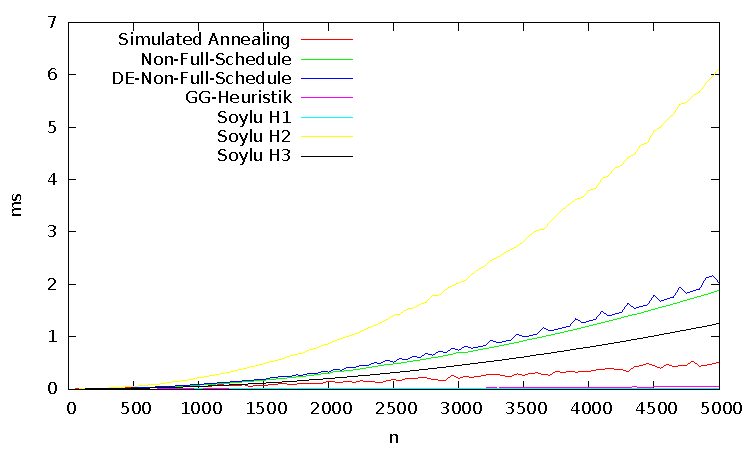
\includegraphics[width=.8\textwidth]{../instances/3dom/plottime.pdf}
    \end{center}
    \caption{
        \label{abb:3domtime}
        Laufzeiten der drei Heuristiken bei drei dominierenden Maschinen (gleichverteilte Prozesszeiten).
    }
\end{figure}

Außerdem ist zu erkennen, dass die Double Ended Non-Full-Schedule-Heuristik fast identische Resultate liefert im Vergleich zur Non-Full-Schedule-Heuristik
und dass die Gilmore-Gomory-Heuristik hier relativ schlechte Resultate liefert und mit Simulated Annealing die besten Lösungen erzeugt werden.
Der Plot der relativen Abweichungen zeigt außerdem, dass diese Abweichungen offenbar nahezu konstant sind zwischen den Heuristiken (nicht beim MIP) 
und nicht von der Instanzgröße abhängen.
Einzig die relative Abweichung des Simulated Annealings scheint mit zunehmender Instanzgröße leicht abzunehmen.

In Abbildung \ref{abb:3domtime} sind die Zeiten aufgetragen, die die Heuristiken benötigten, um die in Abbildung \ref{abb:3dom} dargestellten Resultate zu berechnen.
Deutlich zu erkennen ist der quadratische Anstieg der beiden Non-Full-Schedule-Heuristiken, wobei die Double Ended Variante etwas langsamer ist,
da pro Iteration immer zwei Jobs statt nur einem gesucht werden.
Außerdem treten in der Kurve der Double Ended Non-Full-Schedule-Heuristik teilweise kleine Ausreißer nach oben auf.
Eine plausible Begründung hierfür konnte nicht gefunden werden.
Die Kurve des Simulated Annealings ist, wie zu erwarten war, sehr chaotisch, was durch die nicht deterministische Funktionsweise des Algorithmus erklärt werden kann:
Die Laufzeit hängt stark vom Zufall ab und nur zweitrangig von der Instanzgröße.
Am schnellsten ist die Gilmore-Gomory-Heuristik, die dafür aber auch vergleichsweise schlechte Resultate liefert.

Die zweite Testreihe unterscheidet sich nur dadurch von der ersten, dass die Prozesszeiten der dominierenden Maschinen nicht gleichverteilt aus dem Intervall
$[10,100]$ ausgewählt wurden, sondern normalverteilt mit einem Erwartungswert von $\mu=50$ und einer Standardabweichung von $\sigma=20$.
Die Resultate sind analog zur ersten Testreihe in Abbildung \ref{abb:3domnorm} dargestellt und die Laufzeiten dazu in Abbildung \ref{abb:3domnormtime}.
\begin{figure}
    \begin{center}
        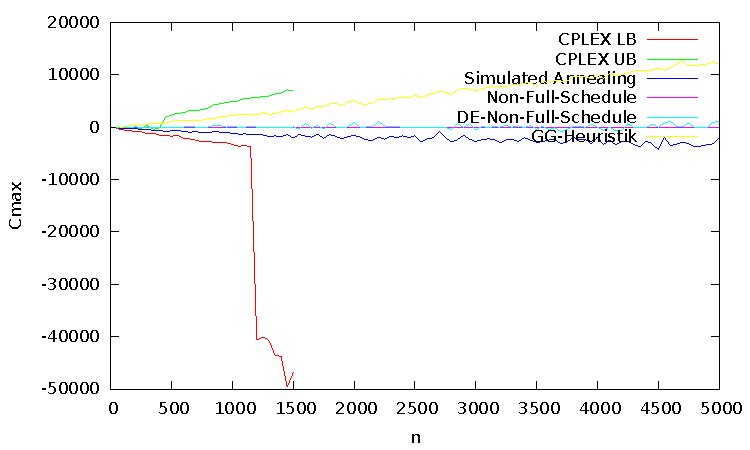
\includegraphics[width=.8\textwidth]{../instances/3dom_norm/plot.pdf}
    \end{center}
    \begin{center}
        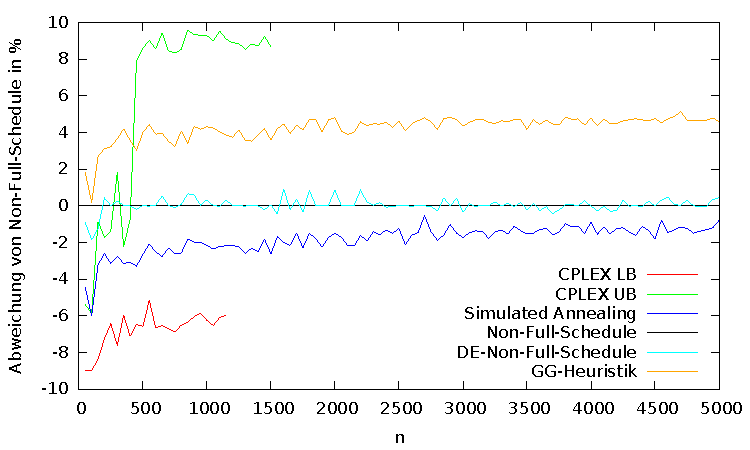
\includegraphics[width=.8\textwidth]{../instances/3dom_norm/plotrel.pdf}
    \end{center}
    \caption{
        \label{abb:3domnorm}
        Absolute (oben) und relative (unten) Unterschiede zwischen der Non-Full-Schedule-Heuristik und den übrigen Heuristiken
        bei drei dominierenden Maschinen (normalverteilte Prozesszeiten).
    }
\end{figure}
\begin{figure}
    \begin{center}
        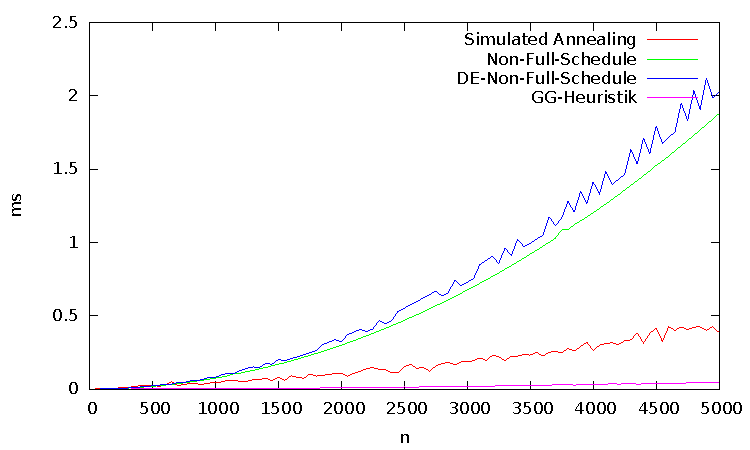
\includegraphics[width=.8\textwidth]{../instances/3dom_norm/plottime.pdf}
    \end{center}
    \caption{
        \label{abb:3domnormtime}
        Laufzeiten der drei Heuristiken bei drei dominierenden Maschinen (normalverteilte Prozesszeiten).
    }
\end{figure}

Die Laufzeiten der zweiten Testreihe unterscheiden nur marginal von denen der ersten, was zu erwarten war, 
da die Laufzeiten der Heuristiken nicht von den Prozesszeiten abhängig sind.
Die Kurven in Abbildung \ref{abb:3domnorm} unterscheiden sich im Verlauf kaum von denen in Abbildung \ref{abb:3dom}.
Allerdings sind diese Kurven im Vergleich zur ersten Testreihe in etwa um den Faktor $2$ gestaucht.
Die Resultate der Heuristiken unterscheiden sich hier also weniger.
Das muss daran liegen, dass die Prozesszeiten (da sie normalverteilt sind) weniger unterschiedlich sind.
Die beiden Non-Full-Schedule-Heuristiken ziehen daraus einen Vorteil, da sie nach eben diesem Prinzip vorgehen, möglichst ähnliche Prozesszeiten zu finden.
Auch die Gilmore-Gomory-Heuristik profitiert davon, da beim (theoretischen) Wiederhochskalieren der Prozesszeiten der dritten dominierenden Maschine 
nur vergleichsweise wenige Zykluszeiten mit vergrößert werden müssen.
Und auch CPLEX kommt bei diesen Daten offenbar ebenfalls schneller zu besseren Schranken.

Die dritte und letzte Testreihe wurde mit einem identischen Verfahren wie die zweite Testreihe generiert.
Allerdings wurde der Erwartungswert der Prozesszeiten auf Maschine $M_3$ auf $\mu=30$ festgesetzt, also um $20$ weniger gegenüber $M_4$ und $M_5$.
Ziel sollte es sein, dass $M_4$ und $M_5$ nicht dominierend sind, sondern nur eine geringe Semidominanz haben, 
so dass die Vorzüge der Gilmore-Gomory-Heuristik zum Tragen kommen.
\begin{figure}
    \begin{center}
        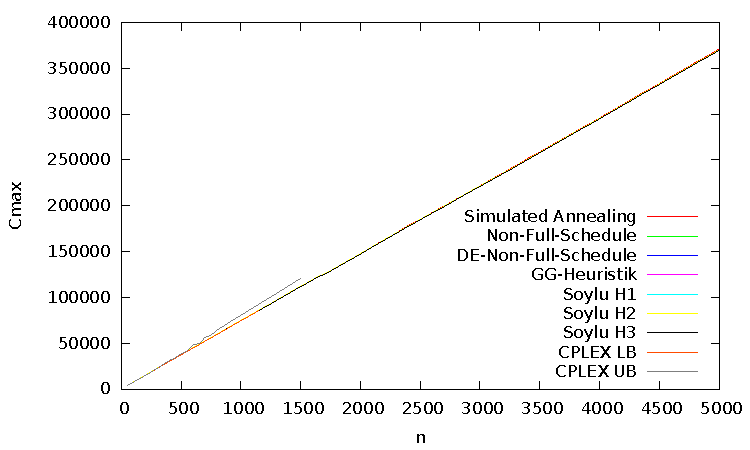
\includegraphics[width=.8\textwidth]{../instances/2quasidom/plot.pdf}
    \end{center}
    \begin{center}
        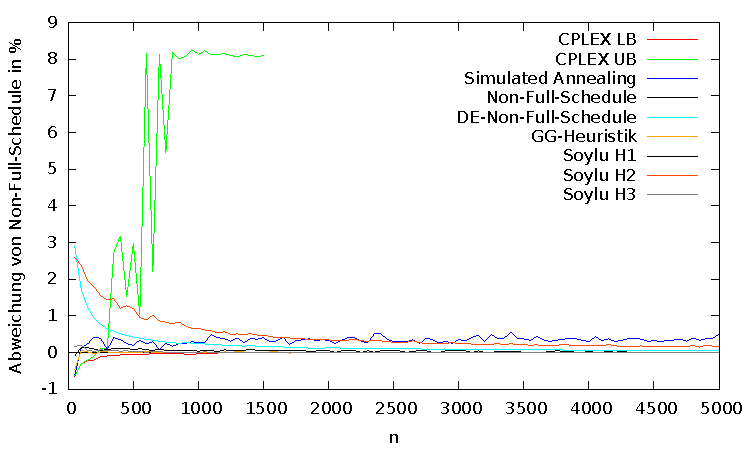
\includegraphics[width=.8\textwidth]{../instances/2quasidom/plotrel.pdf}
    \end{center}
    \caption{
        \label{abb:2quasidom}
        Absolute (oben) und relative (unten) Unterschiede zwischen der Non-Full-Schedule-Heuristik und den übrigen Heuristiken
        bei zwei semidominierenden Maschinen (normalverteilte Prozesszeiten).
    }
\end{figure}
\begin{figure}
    \begin{center}
        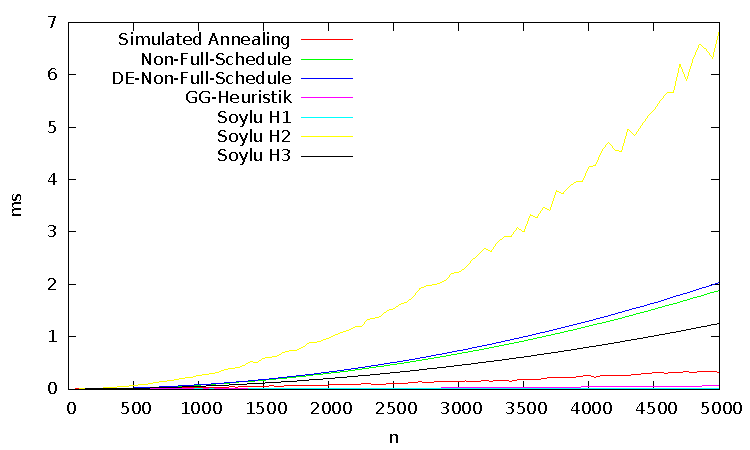
\includegraphics[width=.8\textwidth]{../instances/2quasidom/plottime.pdf}
    \end{center}
    \caption{
        \label{abb:2quasidomtime}
        Laufzeiten der drei Heuristiken bei zwei semidominierenden Maschinen (normalverteilte Prozesszeiten).
    }
\end{figure}

Und tatsächlich bestätigen die Rechenergebnisse diese Vermutung, wie in Abbildung \ref{abb:2quasidom} zu sehen ist.
Fast alle Heuristiken liefern bessere Ergebnisse als sie es bei den ersten beiden Testreihen tun (in der gleichen Zeit, s. Abbildung \ref{abb:2quasidomtime}).
Simulated Annealing ist hier allerdings nicht mehr die beste Heuristik.
Die besten Resultate liefern hier die Gilmore-Gomory-Heuristik, die die größte Verbesserung gegenüber den anderen Testreihen erfährt, 
und die Non-Full-Schedule-Heuristik. Die Resultate von beiden sind nahezu identisch.
Die Double Ended Non-Full-Schedule-Heuristik ist hier bei allen Instanzen schlechter als die Non-Full-Schedule-Heuristik, wenn auch nur um weniger als $1\%$
bzw. bis zu $3\%$ bei sehr kleinen Instanzen.
Bemerkenswert ist außerdem, dass die untere Schranke, die von CPLEX für Instanzen mit $n\leq 1500$ berechnet wurde,
oft bis an die Ergebnisse der Gilmore-Gomory- und der Non-Full-Schedule-Heuristik heranreicht.
Das bedeutet, dass die Resultate dieser beiden Heuristiken nahezu optimal sind.
Andererseits sind die oberen Schranken von CPLEX vergleichsweise weit von den Resultaten der Heuristiken entfernt.
Als Ausblick könnten diese Heuristiken daher in CPLEX integriert werden, um die oberen Schranken zu verbessern.



\section{Zuweisung von Ressourcen}
\label{sec:ZuweisungVonRessourcen}
In diesem Abschnitt geht es darum, den Jobs in der Reihenfolge $\pi$, die in Abschnitt \ref{sec:BerechnenEinerJobreihenfolge} aufgestellt wurde,
Ressourcen zuzuweisen. An diese Zuweisung werden zwei Anforderungen gestellt:
\begin{enumerate}
    \item Die Zuweisung muss zulässig sein. Das heißt, ist eine Ressource einem Job zugewiesen, darf sie den nachfolgenden $m-1$ Jobs nicht mehr zugewiesen werden.
        Das Problem der Zulässigkeit einer Zuweisung wird im ersten Unterabschnitt \ref{subsec:ZulaessigkeitDerZuweisung} betrachtet.
    \item Die Zuweisung soll möglichst gut sein. Wenn zwei Jobs, die im Abstand von $m$ in $\pi$ liegen, die selbe Ressource benutzen können,
        werden Rüstkosten eingespart, da die Ressource nicht ausgetauscht werden muss.
        Dieses Problem wird in Unterabschnitt \ref{subsec:OptimierungDerRessourcenzuweisung} diskutiert.
\end{enumerate}
Es ist natürlich möglich, dass bei gegebenem $\pi$ keine zulässige Zuweisung von Ressourcen möglich ist.
In diesem Fall muss $\pi$ nachträglich geändert werden, worauf in Unterabschnitt \ref{UnzulaessigeReihenfolgen} eingegangen wird.

\subsection{Zulässigkeit der Zuweisung}
\label{subsec:ZulaessigkeitDerZuweisung}
Abhängig davon, welche Ressourcen für welche Jobs geeignet sind, kann das Zulässigkeitsproblem unterschiedlich schwer zu lösen sein.
Folgende Situationen werden betrachtet:
\begin{itemize}
    \item Alle Ressourcen sind für alle Jobs geeignet (trivial, es müssen $m$ Ressourcen vorhanden sein).
    \item Die Ressourcenmengen sind disjunkt ($\rho_i\cap\rho_j \neq \emptyset \enspace \Rightarrow \enspace \rho_i = \rho_j$).
    \item Die Ressourcen sind für hierarchische Jobgruppen geeignet 
        ($\iota_q\cap\iota_r \neq \emptyset \enspace \Rightarrow \enspace \iota_q\subseteq\iota_r$ oder $\iota_r\subseteq\iota_q$).
    \item Die $\rho_i$ sind beliebige Teilmengen von $R$.
\end{itemize}

\subsubsection{Zulässigkeit bei disjunkten Ressourcenmengen}
\label{subsubsec:ZulaessigkeitBeiDisjunktenRessourcenmengen}
Bei disjunkten Ressourcenmengen können die Jobs in Gruppen unterteilt werden, 
so dass zu jeder Jobgruppe eine für sie exklusive Menge an zulässigen Ressourcen zur Verfügung steht.
Für die Zulässigkeit reicht es aus, statt der Ressourcenmengen $\rho_i$ nur deren Größen $|\rho_i|$ zu betrachten
(bei der Optimierung der Zuteilung ist diese Vereinfachung nicht sinnvoll).
Mit einem Greedy-Algorithmus kann eine gegebene Reihenfolge $\pi$ dann auf Zulässigkeit überprüft werden:
Der Algorithmus durchläuft $\pi$ von vorne nach hinten.
Jede Jobgruppe erhält einen Counter, der mitzählt, wie viele Ressourcen momentan für sie zur Verfügung stehen.
Diese Counter werden zu Beginn mit $|\rho_i|$ initialisiert.
An jeder Position in $\pi$ wird der Counter der zugehörigen Jobgruppe dekrementiert.
Nach $m$ Schritten wird dieser Counter wieder inkrementiert.
Sollte ein Counter einmal negativ werden, gibt es keine zulässige Ressourcenzuteilung.

%\subsubsection{Zulässigkeit bei hierarchischen Jobgruppen}
%Diese Situation kann mit einem ähnlichen Greedy-Algorithmus gelöst werden, wie bei disjunkten Ressourcenmengen.
%Die Ressourcen, die für eine Jobgruppe geeignet sind, können hier allerdings nicht als identisch angesehen werden,
%so dass es genügen würde, wieder nur die Anzahl der Ressourcen zu betrachten.
%Die Ressourcen unterscheiden sich dahingehend voneinander, dass sie für unterschiedlich viele andere Jobs ebenfalls geeignet sind.
%Der Greedy-Algorithmus muss so abgeändert werden, dass er jedem Job in $\pi$ immer die "`speziellste"' aktuell für diesen Job verfügbare Ressource zuweist.
%Soll einem Job $j$ eine Ressource zugeteilt werden, muss unter allen geeigneten Ressourcen $r\in\rho_j$, 
%wobei $r$ nicht schon einem anderen Job zugewiesen sein darf, diejenige mit minimalem $|\iota_r|$ ausgesucht werden.
%
%Dieser abgewandelte Greedy-Algorithmus ist korrekt, denn immer, wenn die Situation auftritt, dass für einen Job $j$ keine Ressource verfügbar ist,
%liegt das daran, dass alle potentiell geeigneten Ressourcen $\rho_j$ bereits an einen der $m-1$ direkten Vorgänger von $j$ vergeben worden sind.
%Sei $f$ das unvollständige Mapping, das der Algorithmus bis zu diesem Punkt aufgestellt hat.
%Sei $F\subseteq N$ die Menge der Vorgänger von $j$, denen eine Ressource $r\in\rho_j$ zugeteilt wurde.
%Angenommen, es existiert ein zulässiges Mapping $f'$, obwohl der Algorithmus $j$ keine Ressource zuweisen kann.
%Dann muss es einen Job $i\in F$ geben mit $f'(i)\not\in\rho_j$.
%Wegen der hierarchischen Eigenschaft muss entweder $\iota_{f'(i)}\subset\iota_{f(i)}$ sein oder $\iota_{f(i)}\subseteq\iota_{f'(i)}$.
%Da $f(i)\not\in\rho_j$ ist (und somit auch $j\not\in\iota_{f'(i)}$),
%muss hier $\iota_{f'(i)}\subset\iota_{f(i)}$ sein, denn sonst wäre $j\in\iota_{f(i)}\subseteq\iota_{f'(i)}$.
%Das wiederum bedeutet, dass auch der Algorithmus dem Job $i$ die speziellere Ressource $f'(i)$ zugewiesen hätte.
%Da er das aber nicht getan hat, muss er sie stattdessen einem der $m-1$ direkten Vorgänger von $i$ zugewiesen haben.
%Sei $h$ dieser Vorgänger von $i$.
%Es ist also $f(h)=f'(i)$ und somit $f'(h)\neq f'(i)$.


\subsubsection{Zulässigkeit bei beliebigen Ressourcenteilmengen}
\label{subsubsec:ZulaessigkeitBeiBeliebigenRessourcenteilmengen}
Es ist nicht bekannt, ob das Problem, zu entscheiden, ob es bei gegebenem $\pi$ und beliebigen Ressourcenmengen ein zulässiges Mapping $f$ gibt, 
$\mathcal{NP}$-vollständig ist oder ob es einen polynomiellen Algorithmus gibt.

Es besteht allerdings die Vermutung, dass es bei konstantem $m$ einen polynomiellen Algorithmus in $n$ gibt. Ein Indiz für diese Vermutung liefert folgendes MIP:
\begin{align}
    \text{max} \quad &0 \label{zulmip:obj} \\
    \text{s.t.}\quad \sum_{r\in\rho_i} x_{ir} &= 1 & i\in N \label{zulmip:1} \\
    x_{ir} + x_{jr} &\leq 1 & i\in N, j=i+1,\ldots,i+m-1 \, ,r\in\rho_i\cap\rho_j \label{zulmip:2} \\
    x_{ir} &\in \{0,1\} & i\in N, r\in\rho_i
\end{align}
O.B.d.A. sei hier $\pi_i=i$, d.h. Job $i$ ist an Position $i$.
Die Binärvariablen $x_{ir}$ geben hier an, ob dem Job $i$ die Ressource $r$ zugeteilt wird.
In diesem Fall ist $x_{ir}=1$ und sonst $x_{ir}=0$.
Die erste Nebenbedingung (\ref{zulmip:1}) bewirkt, dass jedem Job genau eine Ressource zugewiesen wird.
Durch die zweite Nebenbedingung (\ref{zulmip:2}) kann jede Ressource jeweils nur einmal an $m$ aufeinander folgende Jobs vergeben werden.
Eine Zielfunktion ist nicht notwendig, da die Zulässigkeit nur durch die Nebenbedingungen entschieden wird.
Mit diesem MIP können selbst sehr große Instanzen mit $n\approx 100000$ (allerdings mit $m\leq 8$) in weniger als einer Sekunde gelöst werden.

Nebenbedingung (\ref{zulmip:2}) verhindert immer nur für Paare von Jobs, deren Abstand kleiner als $m$ ist, dass ihnen die selbe Ressource zugewiesen wird.
Das ist für die Korrektheit des MIPs zwar ausreichend, durch zusätzliche Nebenbedingungen, die dasselbe für Tripel, Quadrupel, bis hin zu $m$-Tupeln verhindern,
können aber einige fraktionale Lösungen der Relaxation "`abgeschnitten"' werden.
Für ein $k$-Tupel von Jobs, die alle in einem Abschnitt von $\pi$ der Länge $m$ stehen, sieht diese zusätzliche Nebenbedingung so aus:
\begin{align}
    \sum_{l=1}^k x_{i_lr} \leq 1 \quad i_l\in N, i_1<i_2<\ldots<i_k<i_1+m, r\in\bigcap_{l=1}^k \rho_{i_l}
\end{align}
Für $k=2$ ist diese Nebenbedingung identisch mit (\ref{zulmip:2}).
Die Anzahl dieser Nebenbedingungen lässt sich durch $\mathcal{O}(n(m-1)!|R|)$ abschätzen, was bei konstantem $m$ polynomiell ist.
Werden sie für $k=3,\ldots,m$ zu obigem MIP hinzugefügt, so war bei allen bislang getesteten Instanzen die Relaxation bereits ganzzahlig.
Ein Beweis, dass dies tatsächlich bei allen Instanzen der Fall ist, ist noch nicht gelungen.
Gelingt er, ist bewiesen, dass es in polynomieller Zeit (bei konstantem $m$) möglich ist, zu entscheiden, ob es für eine gegebene Jobreihenfolge $\pi$ und 
gegebene (beliebige) Ressourcenteilmengen $\rho_i$ möglich ist, allen Jobs eine Ressource zuzuweisen.


\subsection{Optimierung der Ressourcenzuweisung}
\label{subsec:OptimierungDerRessourcenzuweisung}
Da unbekannt ist, ob das Finden \textit{irgendeiner} Ressourcenzuweisung $\mathcal{NP}$-schwer ist,
ist es natürlich ebenfalls unbekannt, ob das Finden einer \textit{optimalen} Ressourcenzuweisung $\mathcal{NP}$-schwer ist.

Eine Ausnahme bildet der Fall von disjunkten Ressourcenteilmengen $\rho_i$.
Immer, wenn zwei Jobs aus einer Familie im Abstand $m$ aufeinander folgen, kann ihnen dieselbe Ressource zugewiesen werden.
Wenn zwei Jobs im Abstand $m$ nicht zur selben Familie gehören, gibt es auch keine Möglichkeit, Rüstkosten zu vermeiden oder zu verringern.

Für den allgemeinen Fall lässt sich das MIP aus Unterabschnitt \ref{subsubsec:ZulaessigkeitBeiBeliebigenRessourcenteilmengen} erweitern:
\begin{align}
    \text{max} \quad \sum_{i=m}^n\sum_{r\in\rho_i\cap\rho_{i-m}} &y_{ir} \label{optmip:obj} \\
    \text{s.t.}\quad \sum_{r\in\rho_i} x_{ir} &= 1 & i\in N \label{optmip:1} \\
    x_{ir} + x_{jr} &\leq 1 & i\in N, j=i+1,\ldots,i+m-1 \, ,r\in\rho_i\cap\rho_j \label{optmip:2} \\
    y_{ir} &\leq x_{ir} & i=m,\ldots,n \, ,r\in\rho_i\cap\rho_{i-m} \label{optmip:3}\\
    y_{ir} &\leq x_{i-m,r} & i=m,\ldots,n \, ,r\in\rho_i\cap\rho_{i-m} \label{optmip:4}\\
    x_{ir} &\in \{0,1\} & i\in N, r\in\rho_i \\
    y_{ir} &\in \{0,1\} & i=m,\ldots,n \, ,r\in\rho_i\cap\rho_{i-m}
\end{align}
Auch hier sei wieder o.B.d.A. $\pi_i=i$.
Für die Binärvariablen $y_{ir}$ gilt $y_{ir}=1$ genau dann, wenn den Jobs an den Positionen $i$ und $i-m$ die selbe Ressource $r$ zugeteilt ist.
Diese Eigenschaft wird durch die Nebenbedingungen (\ref{optmip:3}) und (\ref{optmip:4}) erzwungen.
In der Zielfunktion (\ref{optmip:obj}) wird daher die Anzahl der $y$-Variablen, die auf $1$ gesetzt sind, maximiert, da so die wenigsten Rüstkosten auftreten.
Dieses MIP liefert genau wie jenes aus \ref{subsubsec:ZulaessigkeitBeiBeliebigenRessourcenteilmengen} in weniger als einer Sekunde auch für sehr große Instanzen eine Lösung.
%Dieser Umstand lässt vermuten, dass auch das Optimierungsproblem der Ressourcenzuteilung in polynomieller Zeit lösbar ist.

\section{Unzulässige Reihenfolgen}
\label{UnzulaessigeReihenfolgen}
Für den Fall, dass für eine gegebene Reihenfolge $\pi$ kein zulässiges Mapping $f$ erstellt werden kann, muss $\pi$ nachträglich verändert werden.

%\subsection{Nachbarschaftssuche}
Eine Nachbarschaftssuche ist eine Möglichkeit zur nachträglichen Änderung von $\pi$:
Mit einer Vertauschung zweier Jobs kann $\pi$ unter Umständen so abgeändert werden, dass doch ein zulässiges Mapping existiert.
Der Greedy-Algorithmus aus Unterabschnitt \ref{subsubsec:ZulaessigkeitBeiDisjunktenRessourcenmengen} kann so abgewandelt werden,
dass er, sobald einer der Counter negativ wird, nicht terminiert, sondern weiter Ressourcen zuweist, auch wenn dies eigentlich gar nicht geht.
Sei $j$ ein Job, dessen Counter negativ geworden ist.
Ziel ist es, einen anderen Job $k$ zu finden mit der Eigenschaft, dass die Counter von $j$ und $k$ jeweils noch mindesten $1$ betragen würde, 
wenn man ihre Positionen vertauschen würde,
und dass auch keiner der Counter der umliegenden Jobs von $j$ und $k$ durch eine Vertauschung negativen werden würde.
Falls mehrere solcher $k$ existieren, wird derjenige ausgewählt, dessen Vertauschung mit $j$ die geringste Verschlechterung von $C_{\max}$ verursacht.
Die Counter der umgebenen Jobs müssen nach der Vertauschung aktualisiert werden.
Dieses Vorgehen wird so lange wiederholt, bis es keine negativen Counter mehr gibt.
Falls kein solcher Job $k$ existiert, kann die Zulässigkeit von $\pi$ mit dieser Methode nicht erlangt werden.


%\subsection{Idle-Jobs}
%Falls mit der Nachbarschaftssuche keine Lösung gefunden werden kann, besteht die Möglichkeit sogenannte Idle-Jobs in $\pi$ einzufügen.
%Idle-Jobs sind Jobs, die auf allen Maschinen die Prozesszeit $0$ haben und keine Ressourcen benötigen.
%In der Praxis kann ein Idle-Job durch "`nichts"' realisiert werden, es wird also einfach kein Job in die Station eingelegt.
%Nach dem Einfügen eines Idle-Jobs kann erneut die Nachbarschaftssuche angewandt werden.
%Es können so lange Idle-Jobs eingefügt werden, bis eine gültige Ressourcenzuweisung gefunden wurde.



\chapter{Der zweite Dekompositionsansatz}
In diesem Kapitel wird der zweite Dekompositionsansatz vorgestellt.
Hierbei wird erst jedem Job eine Ressource zugewiesen, also ein Mapping $f$ erzeugt,
und anschließend werden die Jobs in eine Reihenfolge $\pi$ gebracht.
Neben der reinen Ressourcenzuteilung wird im ersten Schritt auch teilweise schon festgelegt, welche Jobs in der späteren Reihenfolge einen Abstand von $m$ haben sollen.
So wird sichergestellt, dass die durch das Mapping $f$ vorgeschriebenen Ressourcenzuteilungen auch dazu führen, dass Rüstkosten eingespart werden.

In Abschnitt \ref{sec:Ressourcenzuweisung} wird erklärt, wie ein optimales Mapping $f$ mit möglichst wenigen Rüstkosten mit einem Binpacking-Ansatz erstellt werden kann.
Anschließend wird in Abschnitt \ref{sec:AnordnungDerJobgruppen} beschrieben, wie basierend auf dem gegebenen Mapping $f$ eine Reihenfolge $\pi$ erstellt wird,
so dass die Summe der Zykluszeiten ($C_{\max}$) minimal ist.

In den meisten nachfolgend genannten Verfahren wird nur der Spezialfall mit konstanten Rüstkosten ($s_{fg}=s$),
disjunkten Ressourcenmengen ($\rho_i\cap\rho_j=\emptyset$) und zwei dominierenden Maschinen betrachtet.


\section{Ressourcenzuweisung}
\label{sec:Ressourcenzuweisung}
In diesem Abschnitt wird die Konstruktion des Mappings $f$ erläutert.
Dabei wird davon ausgegangen, dass Rüstkosten einzig durch einen Ressourcenwechsel verursacht werden.
In Unterabschnitt \ref{subsec:RessourcenzuweisungMitBinpacking} wird auf den Spezialfall $s_{fg}=s$, der mit einem Binpackingansatz gelöst werden kann,
eingegangen.

In realen Anwendungsfällen ist es häufig nicht der Fall, dass bei $n$ zu produzierenden Jobs alle $n$ Jobs unterschiedlich sind,
d.h. unterschiedliche Prozesszeiten und Ressourcen haben.
Stattdessen bietet ein Produzent eine gewisse Anzahl unterschiedlicher Güter an und ein Käufer gibt mehrere identische Güter auf einmal in Auftrag.
Im Folgenden ist daher von \textit{Jobgruppen} die Rede, wobei eine Jobgruppe $g$ aus $n_g\in\mathbb{N}$ identischen Jobs besteht.
$n_g$ ist also die Größe einer Jobgruppe $g$.
Die Anzahl der Jobgruppen wird mit $\tilde{n}$ bezeichnet.
Für die Gesamtanzahl an Jobs gilt dann $n = \sum_{g=1}^{\tilde{n}} n_g$.

%\subsection{Bekannte Laufzeitschranken und Verfahren}
%\label{subsec:BekannteLaufzeitschrankenUndVerfahren}

\subsection{Ressourcenzuweisung mit Binpacking}
\label{subsec:RessourcenzuweisungMitBinpacking}
Bei $\tilde{n}$ gegebenen Jobgruppen, wobei alle Jobs aus einer Gruppe die gleichen Ressourcen verwenden können,
ist es naheliegend, die Jobs einer Gruppe immer im Abstand von $m$ in die Anlage einzulegen.
Auf diese Weise muss die Ressource in der entsprechenden Station so lange nicht ausgetauscht werden,
bis alle Jobs aus einer Jobgruppe fertiggestellt worden sind.
Erst danach, wenn Jobs aus einer anderen Gruppe eingelegt werden, muss einmalig die Ressource gewechselt werden,
so dass nur dann Rüstkosten auftreten.
Dabei soll nur der Spezialfall mit disjunkten Ressourcenmengen und konstanten Rüstkosten ($s_{fg}=s$) betrachtet werden.

O.B.d.A. sei $n$ ein Vielfaches von $m$, denn andernfalls kann eine weitere "`Dummy"'-Jobgruppe $g_d$ konstruiert werden,
deren Jobs die Prozesszeiten $0$ haben und die genau so groß ist, dass $n+n_{g_d}$ ein Vielfaches von $m$ ist.
Bei $\tilde{n}$ gegebenen Jobgruppen mit den Größen $n_g, \, g=1,\ldots,\tilde{n}$ ist das Ziel,
die Jobgruppen in $m$ gleichgroße Teilmengen zu unterteilen, möglichst ohne eine der Jobgruppen zu teilen.
Dieses Problem lässt sich als Binpacking-Instanz betrachten, wobei entschieden werden muss, ob $\tilde{n}$ Items 
mit den Größen $n_1,\ldots,n_{\tilde{n}}$ in $m$ Bins der Größe $\frac{n}{m}$ untergebracht werden können.
Jobs, die sich in einem Bin befinden, werden danach einer Station der Anlage zugewiesen.
Da eine Station sich nach genau $m$ Zyklen wieder an ihrer Ausgangsposition befindet,
werden die Jobs eines Bins immer im Abstand von $m$ in die Anlage eingelegt und wenn sie zur gleichen Jobgruppe gehören, treten keine Rüstkosten auf,
da die Ressource in der Station bleiben kann.

Für den Fall, dass die Binpacking-Instanz eine Lösung hat, müssen noch die Bins den Stationen zugeordnet werden und die Reihenfolge
der Jobgruppen in jedem Bin muss so bestimmt werden, dass die Zykluszeiten minimiert werden.
Dies wird in Abschnitt \ref{sec:AnordnungDerJobgruppen} beschrieben.
Falls dies nicht möglich ist, bedeutet das, dass mindestens eine der Jobgruppen aufgeteilt werden muss auf zwei Bins,
so dass ein weiteres Mal Rüstkosten auftreten.

Um herauszufinden, welche Jobgruppe geteilt werden muss und wie groß die beiden Hälften sein müssen,
wird eine weitere Binpacking-Instanz\footnote{Streng genommen handelt es sich hierbei nicht mehr um eine Binpacking-Instanz wegen der unterschiedlichen Bingrößen.} 
gelöst, die bis auf eine Änderung identisch zur vorherigen ist:
Es gibt nicht mehr $m$ Bins, sondern nur noch $m-1$ und einer dieser Bins hat die Größe $2\frac{n}{m}$ (alle anderen haben weiterhin die Größe $\frac{n}{m}$).
Wenn hier eine Aufteilung möglich ist, kann der Bin mit doppelter Größe wieder halbiert werden,
wobei dann eine der Jobgruppen in ihm auch geteilt werden muss wie in Abbildung \ref{abb:binhalb} veranschaulicht.
Sollte auch hier keine Lösung möglich sein, muss eine weitere Jobgruppe geteilt werden.
Dazu wird wiederum eine neue Binpacking-Instanz erzeugt.
Abbildung \ref{abb:binpart} zeigt, wie die Bingrößen in den weiteren Instanzen aussehen.
Es handelt sich dabei um die \textit{ungeordnete Zahlenpartition} von $m$.
Spätestens bei der Binpacking-Instanz, die nur noch einen Bin enthält mit der Größe $n$, gibt es eine Lösung,
bei der dann $m-1$ Jobgruppen aufgeteilt werden müssen, so dass $m-1$ weitere Ressourcenwechsel und damit Rüstkosten auftreten.
\begin{figure}
    \begin{center}
        \begin{tabular}{cccccccc}
            1 & 1 & 1 & 1 & 1 & 1 & 1 & 1  \\ \hline
            2 & 1 & 1 & 1 & 1 & 1 & 1 & \\ \hline
            2 & 2 & 1 & 1 & 1 & 1 & &\\
            3 & 1 & 1 & 1 & 1 & 1 & &\\ \hline
            2 & 2 & 2 & 1 & 1 & & &\\
            3 & 2 & 1 & 1 & 1 & & &\\
            4 & 1 & 1 & 1 & 1 & & &\\ \hline
            2 & 2 & 2 & 2 & & & &\\
            3 & 2 & 2 & 1 & & & &\\
            3 & 3 & 1 & 1 & & & &\\
            4 & 2 & 1 & 1 & & & &\\
            5 & 1 & 1 & 1 & & & &\\ \hline
            3 & 3 & 2 & & & & &\\
            4 & 2 & 2 & & & & &\\
            4 & 3 & 1 & & & & &\\
            5 & 2 & 1 & & & & &\\
            6 & 1 & 1 & & & & &\\ \hline
            4 & 4 & & & & & &\\
            5 & 3 & & & & & &\\
            6 & 2 & & & & & &\\
            7 & 1 & & & & & &\\ \hline
            8 & & & & & & &
        \end{tabular}
    \end{center}
    \caption{
        \label{abb:binpart}
        Ungeordnete Zahlenpartition von $8$ bezüglich $m'$ gruppiert und sortiert.
        Jede Zeile stellt die Anzahl der Bins und deren Größe bei möglichen Binpacking-Instanzen dar.
    }
\end{figure}

Das Binpacking-Problem ist zwar $\mathcal{NP}$-vollständig, da aber sowohl die Anzahl der Bins $m$ 
als auch die Anzahl der Items bzw. Jobgruppen $\tilde{n}$ meist relativ klein sind (meist deutlich kleiner als die Anzahl Jobs $n$),
lässt sich das Problem, die Jobgruppen den Bins zuzuordnen und ggf. geeignete Jobgruppen zu finden, die aufgeteilt werden müssen, 
trotzdem in hinnehmbarer Zeit mit dem nachfolgenden MIP lösen. 
Für die Binärvariablen $x_{gj}$ gilt: $x_{gj}=1$ genau dann, wenn Jobgruppe $g$ Bin $j$ zugeordnet wird.
Die erste Nebenbedingung fordert, dass jede Jobgruppe in genau einem Bin ist 
und die zweite Nebenbedingung verlangt, dass jeder Bin exakt gefüllt ist.
Dabei sind $B_j$ die Größen der Bins, die zusammen mit der Anzahl der Bins $m'$ mit jedem Aufruf einer Zahlenpartition von $m$ entsprechen:
\begin{align}
    \text{max} \quad &0 \\
    \text{s.t.}\quad \sum_{j=1}^{m'} x_{gj} &= 1 &g=1,\ldots,\tilde{n}\\
    \sum_{g=1}^{\tilde{n}} n_g x_{gj} &= B_j &j=1,\ldots,m' \\
    x_{gj} &\in \{0,1\} &g=1,\ldots,\tilde{n}, \, j=1,\ldots,m'
\end{align}
In Abbildung \ref{abb:binzeit} sind die Laufzeiten dieses MIPs aufgetragen.
Dabei wurde das MIP in ZIMPL formuliert und mit CPLEX gelöst.
Die Partitionen von $m$ wurden der Reihenfolge nach (vgl. Abbildung \ref{abb:binpart}) mit kleiner werdendem $m'$ durchlaufen,
bis eine zulässige Aufteilung gefunden wurde.


\subsection{Zulässigkeit der Zuweisung}
\label{subsec:ZulaessigkeitDerZuweisung}
In Unterabschnitt \ref{subsec:RessourcenzuweisungMitBinpacking} wurde erläutert, wie Jobs bzw. Jobgruppen so angeordnet werden können,
dass möglichst selten eine Ressource gewechselt werden muss, was Rüstkosten verursacht.
Es wurde allerdings davon ausgegangen, dass immer genug Ressourcen vorhanden sind,
d.h. es wurde nur optimiert, ohne zu beachten, ob diese Zuweisung von Ressourcen überhaupt zulässig ist.
Für den Fall der disjunkten Ressourcenmengen wird im Folgenden beschrieben, unter welchen Umständen die Lösung des Binpackings zulässig ist
bezüglich der vorhandenen Ressourcen.
Dazu wird zunächst beschrieben unter welchen Voraussetzungen eine Unzulässigkeit überhaupt nur auftreten kann.
Anschließend wird erläutert, wie selbst dann teilweise doch noch Zulässigkeit erreicht werden kann.

\subsubsection{Voraussetzungen für Unzulässigkeit}
O.B.d.A. kann davon ausgegangen werden, dass es für jede Jobgruppe mindestens eine zulässige Ressource gibt.
Andernfalls könnten diese Jobs niemals produziert werden.
Unzulässigkeit tritt genau dann auf, wenn weniger Ressourcen für eine Jobgruppe $g$ vorhanden sind als sich Jobs aus $g$ gleichzeitig in der Anlage befinden.
Grundvoraussetzung dafür ist, dass $g$ beim Binpacking auf mehrere Bins aufgeteilt wurde.
Ist dies nicht der Fall, werden die Jobs aus $g$ immer im Abstand von $m$ in die Anlage eingelegt,
so dass nur genau eine Ressource benötigt wird, um alle Jobs aus $g$ zu produzieren.
Eine Jobgruppe, die nicht geteilt wird, kann also keine Unzulässigkeit verursachen.
Es müssen daher nur geteilte Jobgruppen betrachtet werden, von denen es maximal $m-1$ geben kann.

Nun soll der Fall betrachtet werden, dass eine Jobgruppe mehrfach geteilt wurde 
(die Gesamtanzahl von Teilungen von allen Jobgruppen zusammen kann höchstens $m-1$ betragen).
Eine Jobgruppe $g$ kann nur dann mehr als einmal geteilt werden, wenn $n_g > \frac{n}{m}$ ist.
Bei einer $k$-fachen Teilung von $g$ gilt für die resultierenden Teilgruppen $n_{g_1},n_{g_k}\leq\frac{n}{m}$ und $n_{g_i}=\frac{n}{m}$ für $i=2,\ldots,k-1$
(vgl. Abbildung \ref{kteilung}).
Allen Teilgruppen mit $g_i=\frac{n}{m}$ kann eine Ressource fest zugeteilt werden, da sich Jobs dieser Teilgruppen durchgehend auf einer Station befinden.
Sie können daher als eigenständige Jobgruppen mit genau einer zulässigen Ressource aufgefasst werden.
Für $g_1$ und $g_k$ stehen dann entsprechend weniger Ressourcen zur Verfügung.
Daher kann o.B.d.A. davon ausgegangen werden, dass jede Jobgruppe höchstens einmal geteilt werden kann, d.h. $k\leq 1$.

Die Lösung des Binpackings kann also nur dann unzulässig sein, wenn es für eine Jobgruppe $g$, die geteilt wird, nur eine Ressource gibt.
Denn wenn es für $g$ mehr als eine Ressource gibt, ist es kein Problem, wenn zwei Jobs aus $g$ gleichzeitig in der Anlage sind.

\subsubsection{Anordnen der Jobgruppen vor der Teilung}
Im vorigen Unterabschnitt wurde festgestellt, dass eine geteilte Jobgruppe nur dann
zu Unzulässigkeit führen kann, wenn es für sie nur eine Ressource gibt.
Wenn ein Bin der Größe $B_j = k\frac{n}{m}$ (im Folgenden ein $k$\textit{-Bin} genannt) 
mit den ihm zugewiesenen Jobgruppen aufgeteilt wird in $k$ Bins der Größe $\frac{n}{m}$, 
stellt sich daher die Frage, ob es möglich ist, die Jobgruppen des $k$-Bins vorher so Anzuordnen, dass sich nur solche Jobgruppen an den "`Bruchstellen"' befinden, 
für die es mehr als eine Ressource gibt (vgl. Abbildung \ref{bruchstelle}), denn dann wäre die Lösung auf jeden Fall zulässig.

\begin{satz}
    Das Problem zu entscheiden, ob die Jobgruppen in einem $k$-Bin (mit $k>1$) so angeordnet werden können,
    dass beim Zerlegen des $k$-Bins in $1$-Bins nur Jobgruppen mit mindestens zwei Ressourcen geteilt werden, ist $\mathcal{NP}$-vollständig.
\end{satz}
\begin{proof}
    Dieses Problem liegt trivialer Weise in $\mathcal{NP}$.
    Es muss also nur noch ein $\mathcal{NP}$-vollständiges Problem darauf reduziert werden.
    Es folgt die Reduktion des \textit{Partition}-Problems:
    Gegeben sei eine Instanz $J$ des \textit{Partition}-Problems mit Zahlen $a_1,\ldots,a_n$.
    Es sei $A\coloneqq\sum_{i=1}^{n}a_i$.
    Es wird eine Instanz $J'$ des gegebenen Problems erstellt mit $n+1$ Jobgruppen und einem $2$-Bin der Größe $A+2$.
    Es wird $g_i \coloneqq a_i$ für $1\leq i\leq n$ gesetzt und $g_{n+1}\coloneqq 2$.
    Für die Jobgruppen $1$ bis $n$ gibt es eine Ressource und für die die Jobgruppe $n+1$ gibt es zwei Ressourcen.
    Die Jobgruppen müssen also so angeordnet werden, dass $n+1$ geteilt wird.
    Die resultierenden $1$-Bins haben dann jeweils die Größe $\frac{A}{2}+1$ und enthalten jeweils eine Jobgruppe der Größe $1$, die aus $n+1$ hervorgehen.

    "`$\Rightarrow$"': $J$ habe eine Lösung, nämlich eine Teilmenge $T\subseteq\{1,\ldots,n\}$ mit $\sum_{i\in T}a_i = \frac{A}{2}$.
    Dann hat auch $J'$ eine Lösung: Alle $g\in T$ werden dem ersten $1$-Bin zugewiesen und alle $g\in\{1,\ldots,n\}\setminus T$ dem zweiten.
    In beiden $1$-Bins ist dann noch genau für eine Jobgruppe der Größe $1$ Platz, sodass jeweils eine Hälfte der Gruppe $n+1$ diesen ausfüllen kann.

    "`$\Leftarrow$"': Habe nun umgekehrt $J'$ eine Lösung. Da jeder $1$-Bin eine Jobgruppe der Größe $1$ enthält, die aus $n+1$ hervorgegangen ist,
    müssen in beiden $1$-Bins die restlichen Jobgruppen zusammen die Größe $\frac{A}{2}$ haben.
    Diese Jobgruppen sind dann auch eine Lösung für $J$.
\end{proof}

In der Praxis kommt es allerdings selten vor, dass es nur eine Jobgruppe mit mehr als einer Ressource gibt.
Je mehr Jobgruppen mehr als eine Ressource haben, desto einfacher wird das Problem.
Der Fall, dass es keine Jobgruppe mit nur einer Ressource gibt ist trivial, da alle Jobgruppen ohne Bedenken geteilt werden können.

\subsubsection{Keine geeignete Anordnung möglich}
Es bleibt noch der Fall zu klären, dass in einem $k$-Bin keine geeignete Reihenfolge der Jobgruppen gefunden werden kann.
Es wird also mindestens eine Jobgruppe $g$ geteilt, obwohl es nur eine Ressource für sie gibt.

Falls $n_g \leq \frac{n}{m}$ ist, ist es immer möglich, die beiden Teilgruppen, die aus $g$ hervorgehen,
so in den Bins anzuordnen, dass niemals zwei Jobs aus $g$ zur gleichen Zeit in der Anlage sind, indem beispielsweise
$g_1$ an den Anfang ihres Bins gelegt wird und $g_2$ ans Ende von ihrem Bin (vgl. Abbildung \ref{abb:blabla}).
Falls mehrere Jobgruppen mit $n_g \leq \frac{n}{m}$ geteilt werden (es können höchstens $m-1$ sein), können in jedem Bin höchstens zwei resultierende 
Teilgruppen vorkommen, so dass es immer möglich ist, eine von beiden an den Anfang und die andere an das Ende des Bins zu legen (vgl. Abbildung \ref{abb:bla}).
Diese Bedingungen, dass die resultierenden Teilgruppen sich nicht \textit{überlappen} (vgl. Abbildung \ref{ueberlappen}) dürfen, 
muss allerdings in den nachfolgenden Verfahren, die $C_{\max}$ minimieren (s. Abschnitt \ref{sec:AnordnungDerJobgruppen}), beachtet werden.
Alternativ kann das Binpacking wiederholt werden, falls es mehrere unterschiedliche Lösungen für eine Instanz gibt. 
Dort werden dann ggf. andere Jobgruppen geteilt, so dass es evtl. keine möglichen Unzulässigkeiten mehr gibt.
Falls keine davon eine bessere Lösung liefert, kann die nächsten Zahlenpartition von $m$ getestet werden.
Je nachdem, ob in der nächsten Zahlenpartition $m'$ verringert wird (vgl. Abbildung \ref{abb:binpart}),
wird dadurch allerdings eine weitere Jobgruppenteilung und damit ein weiteres Mal Rüstkosten in Kauf genommen.

Wenn $n_g > \frac{n}{m}$ ist,
gibt es keine Möglichkeit, $g$ so aufzuteilen, 
dass sich in jedem Zyklus höchstens ein Job aus $g$ in der Anlage befindet,
da nur $\frac{n}{m}$ Zyklen gemacht werden. 
Da $g$ zu groß ist für einen Bin, muss $g$ aber zwangsweise irgendwo geteilt werden, so dass bei nur einer geeigneten Ressource definitiv keine zulässige Lösung existiert.
Dieser Umstand kann aber bereits im Voraus geprüft werden, so dass dieser Fall hier o.B.d.A. nicht auftritt.

\subsubsection{Zusammenfassung}
Insgesamt kann also nur sehr selten keine zulässige Ressourcenzuweisung gefunden werden.
Unzulässige Fälle sind häufig unabhängig von der Zuweisung der Jobgruppen an die Bins und können bereits im Voraus erkannt werden.
Da im Zweifelsfall sämtliche Lösungen von allen Zahlenpartitionen beim Binpacking durchprobiert werden, ist es ausgeschlossen, dass eine Lösung,
bei der nur solche Jobgruppen mit mehr als zwei Ressourcen geteilt werden, nicht gefunden wird, obwohl sie existiert.
Falls tatsächlich keine solche Lösung existiert, gibt es noch die Möglichkeit, in den nachfolgenden Verfahren mit zusätzlichen Nebenbedingungen darauf zu achten,
dass Teilgruppen sich nicht überlappen.


\section{Anordnung der Jobgruppen}
\label{sec:AnordnungDerJobgruppen}
In diesem Abschnitt werden Verfahren zur Anordnung der Jobgruppen in den Bins einerseits und
zum Zuordnen der Bins zu den Stationen andererseits vorgestellt.
Aus den vorangegangenen Verfahren (vgl. Abschnitt \ref{sec:Ressourcenzuweisung}) ist bekannt, zu welchen Bins die Jobgruppen gehören.
Geteilte Jobgruppen werden hier als eigenständige Gruppen betrachtet.
Auch eventuelle zusätzliche Restriktionen, dass die Teile einer geteilten Jobgruppe sich nicht überschneiden dürfen, sind bekannt.
Ziel ist es, $C_{\max}$ zu minimieren, ohne die Jobgruppen zu teilen und somit die bereits minimierten Rüstkosten zu verändern.


\subsection{MIP mit fixierten Bins}
\label{subsec:MIPMitFixiertenBins}
Hier wird zunächst ein MIP vorgestellt, das lediglich die Jobgruppen in den Bins anordnet.
Die Bins sind dabei bereits fest den Stationen zugeordnet (der erste Bin zur ersten Station usw.).
Dieses MIP ist allerdings nur anwendbar bei zwei dominierenden Maschinen, die nicht notwendiger Weise benachbart sein müssen.
Ein MIP, das auch die Bins untereinander anordnet, d.h. den Stationen zuordnet, wird in Unterabschnitt \ref{subsec:MIPMitFreienBins} vorgestellt.

Die Idee des MIPs besteht darin, jeder Jobgruppe $i$ in ihrem Bin $b_i$ eine \textit{Startposition} $s_i$ zuzuweisen.
Aus der Startposition und der Länge $n_i$ einer Jobgruppe kann ihre \textit{Endposition} bestimmt werden.
Anhand dieser Start- und Endpositionen kann dann die Überlappung $o_{ij}$ mit einer anderen Jobgruppen $j$ aus einem anderen Bin $b_j$
berechnet werden.
Da die Bins den Stationen fest zugeordnet sind und es nur zwei dominierende Maschinen gibt, deren Abstand bekannt ist, 
müssen jeweils nur die Überlappungen von Jobs in Bins mit dem Abstand der dominierenden Maschinen berechnet werden.
Dazu ein Beispiel: Es gebe $m=8$ Maschinen, wobei $M_3$ und $M_4$ dominierend sind. 
Jobgruppe $1$ habe die Größe $n_1=10$ und liege im ersten Bin.
Jobgruppe $2$ habe die Größe $n_2=7$ und liege im zweiten Bin.
Da der Abstand der dominierenden Maschinen $1$ beträgt, wird der zweite Bin als \textit{Nachbarbin} von Bin 1 bezeichnet.
Bin 3 ist der Nachbarbin von Bin 2, Bin 4 ist der Nachbarbin von Bin 3, \ldots und Bin 1 ist der Nachbarbin von Bin 8.
Wenn der Abstand der dominierenden Maschinen hingegen z.B. $3$ betragen würde, dann wäre Bin 4 der Nachbarbin von Bin 1 usw.
Als erstes wird ein Job aus dem ersten Bin in die Anlage eingelegt, dann einer aus dem zweiten usw. 
Die Jobs im ersten Bin werden also immer genau in dem Moment von $M_4$ bearbeitet, wenn die Jobs im zweiten Bin von $M_3$ bearbeitet werden.
Die Startposition von Gruppe $1$ sei nun $s_1=0$ (als allererstes wird also ein Job aus Gruppe $1$ in die Anlage eingelegt)
und die Startposition von Gruppe $2$ sei $s_2=6$.
Die Überlappung der Gruppen $1$ und $2$ beträgt also $4$, wie auch in Abbildung \ref{abb:binfixbsp} zu sehen ist.
D.h. es kommt genau viermal vor, dass ein Job aus Gruppe $1$ von Maschine $M_4$ bearbeitet wird, während ein Job aus Gruppe $2$ von $M_3$ bearbeitet wird.
Da diese beiden Maschinen dominierend sind, beträgt die Zykluszeit in diesen vier Zyklen $\max\{p_{41},p_{32}\}$.

Ziel muss es also sein, den Jobgruppen Startpositionen in ihren Bins zuzuweisen und darauf basierend die Überlappungen mit Gruppen 
aus den Nachbarbins zu berechnen. 
Aus dem Maximum der Prozesszeiten der Jobgruppen und ihren Überlappungen kann dann $C_{\max}$ bestimmt werden.

Die Berechnung der Überlappungen bildet den Kern dieses MIPs.
Es gibt fünf Möglichkeiten, wie sie berechnet werden müssen, die auch in Abbildung \ref{abb:overlap} illustriert sind:
\begin{enumerate}
    \item $o_{ij} = s_i + n_i - s_j$,
    \item $o_{ij} = s_j + n_j - s_i$,
    \item $o_{ij} = n_i$,
    \item $o_{ij} = n_j$ und
    \item $o_{ij} = 0$.
\end{enumerate}
Welche davon die passende ist, muss anhand einiger Hilfsvariablen und Nebenbedingung ermittelt werden.
Außerdem gibt es auch noch den Sonderfall, dass zwischen zwei Nachbarbins der Übergang von Bin $m$ zu Bin $1$ liegt.
Dieser Fall ist in Abbildung \ref{abb:sigma} veranschaulicht.
Wie dort zu sehen ist, muss dann die Berechnung der Überlappung leicht abgeändert werden, da Bin $1$ im Verhältnis zu Bin $m$ um 1 nach oben verschoben scheint.
Die ersten beiden Möglichkeiten zur Berechnung der Überlappung ändern sich dann zu
\begin{enumerate}
    \item $o_{ij} = s_i + n_i + 1 - s_j$ und 
    \item $o_{ij} = s_j + n_j - s_i - 1$.
\end{enumerate}
Die Startpositionen von $i$ werden also jeweils um $1$ nach hinten verschoben, bzw. die von $j$ um $1$ nach vorn.
Zur Vereinfachung wird im MIP ein binärer Parameter $\sigma_{ij}$ benutzt, der genau dann den Wert $1$ hat, wenn dieser Sonderfall eintritt, und sonst $0$.
Auf diese Weise kann $\sigma_{ij}$ direkt in die Berechnung von $o_{ij}$ integriert werden:
\begin{enumerate}
    \item $o_{ij} = s_i + n_i + \sigma_{ij} - s_j$ und 
    \item $o_{ij} = s_j + n_j - s_i - \sigma_{ij}$.
\end{enumerate}

Um festzustellen, welche der Berechnungen für $o_{ij}$ benutzt werden muss, werden binäre Hilfsvariablen $y_{ij}$ und $z_{ij}$ verwendet.
Es ist $y_{ij}=1$ genau dann, wenn $s_j \geq s_i + \sigma_{ij}$ ist, d.h. $j$ "`startet"' gleichzeitig oder später als $i$.
Für $z_{ij}$ gilt in ähnlicher Weise: $z_{ij}=1$ genau dann, wenn $s_i + n_i + \sigma_{ij} \geq s_j + n_j$, 
d.h. die Endposition von $i$ liegt hinter der von $j$ oder gleichauf.
Aus den vier möglichen Kombinationen der Werte von $y_{ij}$ und $z_{ij}$ lässt sich bestimmen, 
welche der ersten vier Berechnungsmöglichkeiten für $o_{ij}$ gewählt werden muss.
Sollte diese Berechnung einen negativen Wert liefern, tritt der fünfte Fall ein.

Im MIP wird mit $\tilde{N}=\{1,\ldots,\tilde{n}\}$ die Menge der Jobgruppen bezeichnet.
$B=\{1,\ldots,m\}$ ist die Menge der Bins und für $b\in B$ ist $\tilde{N}_b\subset \tilde{N}$ die Teilmenge der Jobgruppen, die in Bin $b$ liegen.
Für $i\in\tilde{N}$ gibt $b_i\in B$ den Bin an, in dem sich $i$ befindet.
$\tilde{N}_b^*\subset \tilde{N}$ bezeichnet die Menge der Jobgruppen im Nachbarbin von $b$.
$p_{1i}$ und $p_{2i}$ sind die Prozesszeiten von Jobgruppe $i$ auf der ersten bzw. zweiten dominierenden Maschine.
Für je zwei Jobgruppen $i,j\in N_b$, die im selben Bin $b$ liegen, gibt es
zwei Binärvariablen $x_{ij},x_{ji}$. Es ist $x_{ij}=1$ genau dann, wenn 
Jobgruppe $i$ vor $j$ auf dem Bin liegt. Dabei muss $i$ nicht notwendiger
Weise direkt vor $j$ liegen, sondern an beliebiger Position davor.
Mithilfe der $x_{ij}$ lassen sich die Startpositionen bestimmen:
\begin{align}
    \text{min}\quad &\sum_{b\in B}\sum_{\substack{i\in \tilde{N_b}\\j\in \tilde{N}_b^*}} 
            \max\{p_{2i},p_{1j}\}o_{ij} \label{objfunc1}\\
			\text{s.t.} \quad x_{ij} + x_{ji} &= 1 &i\in \tilde{N}, j\in \tilde{N}_{b_i}, i<j \label{con1:reflex}\\
			x_{ij} + x_{jk} &\leq x_{ik} + 1 &i\in \tilde{N},\,\, j,k\in \tilde{N}_{b_i} \label{con1:transitiv} \\
			s_i &= \sum_{\substack{j\in \tilde{N}_{b_i}\\i\neq j}} n_j x_{ji} &i\in \tilde{N} \label{con1:start} \\
            My_{ij} &\geq s_j - s_i - \sigma_{ij} + \epsilon &i\in \tilde{N}, j\in \tilde{N}^*_{b_i} \label{con1:y1} \\
            M(1-y_{ij}) &\geq s_i - s_j + \sigma_{ij} &i\in \tilde{N}, j\in \tilde{N}^*_{b_i} \label{con1:y2} \\
            Mz_{ij} &\geq s_i + n_i - s_j - n_j + \sigma_{ij} + \epsilon &i\in \tilde{N}, j\in \tilde{N}^*_{b_i} \label{con1:z1} \\
            M(1-z_{ij}) &\geq s_j + n_j- s_i - n_i - \sigma_{ij} &i\in \tilde{N}, j\in \tilde{N}^*_{b_i} \label{con1:z2} \\
            o_{ij} &\geq s_i + n_i - s_j + \sigma_{ij} - M(1-y_{ij}+z_{ij}) &i\in \tilde{N}, j\in \tilde{N}^*_{b_i} \label{con1:o1} \\
            o_{ij} &\geq s_j + n_j - s_i - \sigma_{ij} - M(1-y_{ji}+z_{ji}) &i\in \tilde{N}, j\in \tilde{N}^*_{b_i} \label{con1:o2} \\
            o_{ij} &\geq n_j - M(2-y_{ij}-z_{ij}) &i\in \tilde{N}, j\in \tilde{N}^*_{b_i} \label{con1:o3} \\
            o_{ij} &\geq n_i - M(2-y_{ji}-z_{ji}) &i\in \tilde{N}, j\in \tilde{N}^*_{b_i} \label{con1:o4} \\
            o_{ij} &\geq 0 &i\in \tilde{N}, j\in \tilde{N}^*_{b_i} \label{con1:o5} \\
            x_{ij} &\in \{0,1\} &i\in \tilde{N}, j\in \tilde{N}_{b_i} \\
            y_{ij},z_{ij} &\in \{0,1\} &i\in \tilde{N}, j\in \tilde{N}^*_{b_i}
\end{align}
Mit (\ref{con1:reflex}) wird erreicht, dass immer entweder $i$ vor $j$ liegt
oder umgekehrt. (\ref{con1:transitiv}) stellt die Transitivität dieser Beziehung
her. Auf Grundlage der $x_{ij}$ und der Größen der Jobgruppen $g_i$ 
kann in (\ref{con1:start}) die Startposition jeder Jobgruppe berechnet werden.
Die Variablen $s_i$ dienen dabei nur der Übersicht und können in den übrigen 
Nebenbedingungen durch die Summe aus (\ref{con1:start}) ersetzt werden.
Über (\ref{con1:y1}) und (\ref{con1:y2}) wird den Indikatorvariablen $y_{ij}$ 
mit einem "`Big-M"' die oben beschriebene Bedeutung gegeben:
(\ref{con1:y1}) setzt $y_{ij}$ auf $1$, wenn $s_j-s_i-\sigma_{ij}+\epsilon > 0$ ist,
was äquivalent zu $s_j \geq s_i+\sigma_{ij}$ ist.
$\epsilon$ ist ein hinreichend kleiner Parameter, falls alle Prozesszeiten ganzzahlig sind, ist jeder Wert $\epsilon<1$ geeignet.
(\ref{con1:y2}) andererseits setzt $y_{ij}$ auf $0$, wenn $s_i-s_j+\sigma_{ij} > 0$ ist (oder äquivalent dazu: $s_j < s_i+\sigma_{ij}$).
Analog wird mit (\ref{con1:z1}) und (\ref{con1:z2}) der Wert der $z_{ij}$ entsprechend der obigen Bedeutung gesetzt.
Je nachdem, welche der $y_{ij}$ und $z_{ij}$ auf $1$ bzw. $0$ gesetzt sind, 
werden drei der vier Nebenbedingungen (\ref{con1:o1}) bis (\ref{con1:o4}) durch die "`Big-Ms"' faktisch bedeutungslos ($o_{ij}\geq -M$)
und nur eine bleibt bestehen, so dass genau die passende der vier Berechnungsmöglichkeiten für die $o_{ij}$ gewählt wird.
Da die Zielfunktion (\ref{objfunc1}) die Überlappungen (mit dem Maximum der jeweiligen Prozesszeiten multipliziert) minimiert,
müssen die $o_{ij}$ nicht per Nebenbedingung nach oben beschränkt werden.
Sie sind automatisch durch die Größe der Bins beschränkt.
Damit sie nicht negativ werden, sind sie allerdings durch (\ref{con1:o5}) nach unten durch $0$ beschränkt.
Dies bedeutet, dass die jeweiligen Jobgruppen sich nicht überschneiden.

Die Qualität der Lösung dieses MIPs ist stark von der gegebenen Zuordnung der Bins an die Stationen abhängig.
Bei einigen Zuordnungen kann es sehr gute Lösungen geben, und bei anderen dagegen nur sehr schlechte, was sich nur durch eine
Änderung der Zuordnung (bzw. der Binreihenfolge) verbessern lässt, wozu dieses MIP allerdings nicht in der Lage ist.
Im Folgenden werden daher ein weiteres MIP vorgestellt, das diese Fähigkeit besitzt, und heuristische Methoden,
die die Bins den Stationen zuweisen, um darauf basierend dieses MIP anzuwenden.


\subsection{MIP mit freien Bins}
\label{subsec:MIPMitFreienBins}
Das folgende MIP erweitert das MIP aus Unterabschnitt \ref{subsec:MIPMitFixiertenBins} um die Fähigkeit, die Bins untereinander zu Vertauschen,
was dem Zuweisen der Bins an die Stationen entspricht.
Für die Berechnung der Überschneidungen zwischen den Jobgruppen sind daher weitere Variablen notwendig, die als Indikator dafür dienen,
ob die Bins der Jobgruppen auf benachbarten Stationen liegen.
Dazu dienen die Binärvariablen $\beta_{bd}$, die genau dann auf $1$ gesetzt werden, wenn Bin $b$ Station $d$ zugewiesen ist.
Weitere Binärvariablen $\nu_{bcd}$ werden auf $1$ gesetzt, wenn Bin $b$ Station $d$ zugewiesen ist und Bin $c$ der Nachbarstation von $d$ (mit $d^*$ bezeichnet).
Auf diese Weise können die $\nu_{bcd}$ die $\sigma_{ij}$ aus dem MIP in Unterabschnitt \ref{subsec:MIPMitFixiertenBins} ersetzen:
Wenn die beiden dominierenden Maschinen benachbart sind (also den Abstand $1$ haben), ist für zwei Jobgruppen $i$ und $j$ $\nu_{b_ib_jm}=1$ genau dann, 
wenn der Bin von $i$ der letzten Station $m$ zugewiesen ist und der Bin von $j$ der ersten Station (also genau dann, wenn im anderen MIP $\sigma_{ij}=1$ ist).
Außerdem gibt es weitere Binärvariablen $w_{ij}$, die als Indikator dafür dienen, ob die Bins der Jobgruppen $i$ und $j$ benachbarten Stationen zugewiesen sind.
Denn nur dann muss zwischen diesen Jobgruppen die Überlappung $o_{ij}$ berechnet werden.
\begin{align}
    \text{min}\quad &\sum_{\substack{i,j\in\tilde{N}\\b_i\neq b_j}} 
            \max\{p_{2i},p_{1j}\}o_{ij} \label{objfunc}\\
    \text{s.t.} \quad x_{ij} + x_{ji} &= 1 &i\in\tilde{N}, j\in\tilde{N}_{b_i} 
            \label{con:reflex}\\
    x_{ij} + x_{jk} &\leq x_{ik} + 1 &i\in\tilde{N},\,\, j,k\in\tilde{N}_{b_i} 
            \label{con:transitiv} \\
    s_i &= \sum_{\substack{j\in\tilde{N}_{b_i}\\i\neq j}} g_j x_{ji} &i\in\tilde{N} 
            \label{con:start} \\
	\sum_{b\in B}\beta_{bd} &= 1 &d\in B \label{con:binpos} \\
	\sum_{d\in B}\beta_{bd} &= 1 &b\in B \label{con:binpos2} \\
	\beta_{bd} + \beta_{cd^*} &\leq \nu_{bcd} + 1 &b,c,d\in B \label{con:nu} \\
	\nu_{bcd} &\leq \beta_{bd} &b,c,d\in B \label{con:nurev} \\
    \nu_{bcd} &\leq \beta_{bd^*} &b,c,d\in B \label{con:nurev2} \\
    My_{ij} &\geq s_j - s_i - \nu_{b_ib_jm} + \epsilon &i,j\in\tilde{N} \label{con:y1}\\
    M(1-y_{ij}) &\geq s_i + \nu_{b_ib_jm} - s_j &i,j\in\tilde{N} \\
    Mz_{ij} &\geq s_i + n_i + \nu_{b_ib_jm} - s_j - n_j + \epsilon &i,j\in\tilde{N} \\
    M(1-z_{ij}) &\geq s_j + n_j - s_i - n_i - \nu_{b_ib_jm} &i,j\in\tilde{N} \\
	w_{ij} &= \sum_{d\in B} \nu_{b_ib_jd} &i,j\in\tilde{N} \label{con:w} \\
    o_{ij} &\geq s_i + n_i + \nu_{b_ib_jm} - s_j \notag \\
		   &\phantom{\geq} - M(2-y_{ij}+z_{ij}-w_{ij}) &i,j\in\tilde{N} \label{con:o1} \\
    o_{ij} &\geq s_j + n_j - s_i - \nu_{b_ib_jm} \notag \\
           &\phantom{\geq} - M(2+y_{ij}-z_{ij}-w_{ij}) &i,j\in\tilde{N} \label{con:o2} \\
    o_{ij} &\geq n_j - M(3-y_{ij}-z_{ij}-w_{ij}) &i,j\in\tilde{N} \\
	o_{ij} &\geq n_i - M(1+y_{ij}+z_{ij}-w_{ij}) &i,j\in\tilde{N} \label{con:o4} \\
    o_{ij} &\geq 0 &i,j\in\tilde{N} \\
	\beta_{bd} &\in \{0,1\} &b,d\in B \\
	\nu_{bcd} &\in \{0,1\} &b,c,d\in B, b\neq c \\
    x_{ij} &\in \{0,1\} &i\in\tilde{N},j\in\tilde{N}_{b_i} \\
    y_{ij},z_{ij},w_{ij} &\in \{0,1\} &i,j\in\tilde{N}
\end{align}
Die Nebenbedingungen (\ref{con:binpos}) und (\ref{con:binpos2}) gewährleisten, dass jeder der $m$ Bins genau einer der $m$ Stationen zugewiesen wird.
Über die Nebenbedingungen (\ref{con:nu}), (\ref{con:nurev}) und (\ref{con:nurev2}) wird erzwungen, dass die Binärvariablen
$\nu_{bcd}$ genau dann auf $1$ gesetzt werden, wenn Bin $b$ Station $d$ zugewiesen ist und zugleich Bin $c$ der Nachbarstation $d^*$.
In (\ref{con:w}) wird $w_{ij}$ auf $1$ gesetzt, falls die Bins von $i$ und $j$ benachbarten Stationen zugewiesen sind.
Wenn $w_{ij}=0$ ist, verlieren die Nebenbedingungen (\ref{con:o1}) bis (\ref{con:o4}) ihre Bedeutung.
Davon abgesehen sind diese Nebenbedingungen aber identisch zu denen aus dem MIP im vorherigen Unterabschnitt.
Ähnlich wie die $s_i$ dienen die $w_{ij}$ nur der Übersicht und können durch die Summe in (\ref{con:w}) ersetzt werden.

In dieser Form verlangt das MIP, dass die beiden dominierenden Maschinen benachbart sein müssen.
Denn dann gibt es nur zwei Stationen, zwischen denen die Berechnung der Überlappung um $1$ versetzt stattfinden muss.
Wenn die dominierenden Maschinen beispielsweise einen Abstand von $2$ haben,
tritt dieser Sonderfall der Berechnung sowohl zwischen den Station $m-1$ und $1$ auf als auch zwischen $m$ und $2$,
was durch die Variablen $\nu_{b_i,b_j,m-1}$ bzw. $\nu_{b_ib_jm}$ erkannt werden kann.
Diese müssten dann auch beide in die Nebenbedingungen (\ref{con:y1}) bis (\ref{con:o2}) einfließen.
Da immer höchstens eine von beiden gleichzeitig auf $1$ gesetzt sein kann, 
bewirken dann diese beiden Variablen zusammen die um $1$ versetzte Berechnung der Überlappung.

Das Lösen dieses MIPs mit CPLEX dauert sehr viel länger als beim MIP mit fixierten Bins.
Allerdings ist die obere Schranke, also die aktuell beste gefundene Lösung, meist schon nach wenigen Minuten besser als die
beste Lösung mit fixierten Bins (abhängig davon, ob die gegebene Binreihenfolge dort zufällig "`gut"' ist).

\subsection{Mehrere fixierte Reihenfolgen}
Das MIP in Unterabschnitt \ref{subsec:MIPMitFreienBins} liefert zwar theoretisch optimale Lösungen, diese zu berechnen benötigt aber zu viel Zeit.
Schon bei kleinen Instanzen mit $\tilde{n}=10$ Jobgruppen und $m=8$ beträgt der LP-Gap nach einer Stunde Berechnung noch $20\%$.
Man beachte, dass es bei $10$ Jobgruppen und $8$ Bins mindestens $6$ Bins gibt mit genau einer Jobgruppe.
Es müssen also im Wesentlichen nur noch die Bins den Stationen zugeordnet werden.

Das MIP mit fixierten Bins hingegen findet erst ab Instanzen mit ca. $\tilde{n}=25$ nicht mehr die optimale Lösung innerhalb von einer Stunde.
Je nach Größe der Jobgruppen kann dies ein beträchtlicher Unterschied zu $\tilde{n}=10$ sein. 
Allerdings ist die Güte der Lösungen des MIPs mit fixierten Bins von der initialen Binreihenfolge abhängig.
Dazu wird in diesem Unterabschnitt versucht, solch eine initiale Binreihenfolge zu erzeugen, mit der das MIP dann arbeiten kann.

\subsubsection{Benutzung beider MIPs}
Beobachtungen der Leistung der beiden MIPs haben ergeben, dass das MIP mit freien Bins oft schon nach relativ kurzer Zeit eine bessere obere Schranke
(d.h. die beste bis zu diesem Zeitpunkt gefundene Lösung) liefert als das MIP mit fixierten Bins.
Daher ist ein Ansatz, das MIP mit freien Bins für eine gewisse Zeit laufen zu lassen und dann die Zuteilung der Bins zu den Stationen
auszulesen (diese ist in den $\beta_{bd}$-Variablen kodiert), um anschließend mit dieser Binreihenfolge das MIP mit fixierten Bins zu starten.
%hier noch ein bisschen mehr schreiben...


\subsubsection{Optimum zwischen zwei Bins}
Betrachtet man zwei beliebige Bins $b$ und $c$ auf benachbarten Stationen, ist es möglich, 
all jene Zyklen $t$ zu betrachten, in denen ein Job aus $b$ auf der zweiten dominierenden Maschine ist und ein Job aus $c$ auf der ersten.
Die zugehörigen Zykluszeiten $c_t$ werden dann durch die Prozesszeiten dieser Jobs auf den beiden dominierenden Maschinen definiert (vgl. Abbildung \ref{abb:lokalopt}).
Die Summe dieser Zykluszeiten zwischen zwei benachbarten Bins $b$ und $c$ wird mit $C_{bc}$ bezeichnet.
\begin{satz}
    Seien $b$ und $c$ zwei Bins auf benachbarten Stationen.
    Wenn die Jobgruppen in $b$ absteigend nach ihren Prozesszeiten auf der zweiten dominierenden Maschine angeordnet werden
    und die Jobgruppen in $c$ absteigend nach ihren Prozesszeiten auf der ersten dominierenden Maschine,
    dann ist $C_{bc}$ minimal.
\end{satz}
\begin{proof}
    \textit{hmm...}
\end{proof}
Wenn die Jobgruppen in zwei benachbarten Bins so angeordnet sind, dass $C_{bc}$ minimal ist, wird dieser Wert mit $C_{bc}^*$ bezeichnet.
Dieses Optimum zwischen zwei Bins ist auf die Anordnung aller $m$ Bins übertragen aber nur ein lokales:
Wird ein Bin bezüglich eines seiner Nachbarn in dieser Weise angeordnet, ist es im Allgemeinen nicht der Fall,
dass diese Anordnung auch bezüglich des anderen Nachbarn optimal ist.

In den folgenden Absätzen werden einige Anwendungen dieses lokalen Optimums vorgestellt.

\subsubsection{Bestimmung einer unteren Schranke}
Eine Anwendungsmöglichkeit der lokal optimalen Bins ist die Berechnung einer unteren Schranke für $C_{\max}$ im zweiten Dekompositionsansatz.
Eine mögliche untere Schranke lässt sich wie folgt berechnen:
\[LB_{C_{\max}} = \frac{1}{2} \sum_{b=1}^m \left( \min_{\substack{a=1\\a\neq b}}^m C_{ab}^* + \min_{\substack{c=1\\c\neq b}}^m C_{bc}^* \right) \]
Es werden also für jeden Bin $b$ sein optimaler linker Nachbar $a$ und sein optimaler rechter Nachbar $c$ gesucht.
Da in der Summe all dieser $C_{bc}^*$-Werte jeder Bin zweimal (einmal als linker und einmal als rechter Nachbar) auftaucht,
wird diese Summe noch halbiert.

\subsubsection{Heuristik für initiale Binreihenfolge}
Eine andere mögliche Anwendung der lokal optimalen Bins ist, eine initiale Binreihenfolge (bzw. eine initiale Zuweisung der Bins zu den Stationen)
auf heuristischem Wege zu finden, mit der dann das MIP mit fixierten Bins arbeiten kann.
Als erster Schritt wird unter allen möglichen $C_{bc}^*$-Werten (für alle Bins $b,c$) das Minimum gesucht.
Die zugehörigen Bins $b$ und $c$ werden der ersten Station und der Nachbarstation der ersten Station zugewiesen.
Anschließend wird unter allen noch nicht zugewiesenen Bins derjenige Bin $d$ gesucht, der den besten $C_{cd}^*$-Wert aufweist.
Da $d$ ein "`vielversprechender"' Nachbar für $c$ ist, wird er der Nachbarstation von $c$ zugewiesen.
Dieses Vorgehen wird so lange wiederholt, bis jeder Bin einer Station zugewiesen ist.

Falls der Abstand der dominierenden Maschinen $d_{\mathit{dom}}$($=\text{Abstand benachbarter Stationen}$) und die Anzahl der Maschinen $m$ nicht teilerfremd sind,
gibt es unter den Stationen disjunkte Gruppen, die untereinander nicht durch Nachbarschaft erreicht werden können.
Beispielsweise bilden bei $m=8$ und $d_{\mathit{dom}}=2$ die Stationen $1,3,5,7$ und $2,4,6,8$ solche disjunkten Gruppen.
In diesem Fall muss das obige Verfahren für jede dieser Gruppen separat durchgeführt werden.


\subsection{Nachbarschaftssuche}
Als Alternative zu den MIPs mit freien oder fixierten Bins lassen sich Nachbarschaftsoperatoren beschreiben, 
die für diverse Nachbarschaftssuchverfahren benutzt werden können.
Naheliegende Operatoren sind:
\begin{itemize}
    \item $\mathit{bch}_{bc}$: vertauscht die Bins an den Stationen $b$ und $c$ miteinander,
    \item $\mathit{jch}_{bjk}$: vertauscht im Bin an Station $b$ die Jobgruppen $j$ und $k$ miteinander.
\end{itemize}
Es wurde ein Simulated Annealing Algorithmus implementiert, der diese beiden Nachbarschaften benutzt.
Dieser ähnelt dem Simulated Annealing aus Abschnitt \ref{subsubsec:Nachbarschaftssuche} und unterscheidet sich bloß in einem Punkt von diesem:
In jeder Iteration wird mit einer Wahrscheinlichkeit von $\frac{m}{\tilde{n}+m}$ eine neue Lösung aus der $\mathit{bch}_{bc}$-Nachbarschaft erzeugt 
(mit zufällig gewählten $b$ und $c$) und mit einer Wahrscheinlichkeit von $\frac{\tilde{n}}{\tilde{n}+m}$ eine Lösung aus der $\mathit{jch}_{bjk}$-Nachbarschaft
(mit ebenfalls zufälligen $b,j,k$).
Auf diese Weise wird je nach Verhältnis zwischen der Anzahl der Jobgruppen ($\tilde{n}$) und der Bins ($m$) der entsprechende Operator häufiger benutzt.

Im Gegensatz zu den beiden MIPs ist dieser heuristische Lösungsansatz nicht darauf angewiesen, dass nur zwei Maschinen dominierend sind.


\chapter{Rechenergebnisse und Vergleiche}
\textit{Anfang September anfangen, soweit Messergebnisse vorliegen.}

Obwohl in den vorherigen Kapiteln schon einige Laufzeiten vorgestellt werden, hier nochmal eine Zusammenfassung und insbesondere ein Vergleich
zwischen den beiden Dekompositionsansätzen. Sowohl echte Instanzen als auch generierte. 
Dabei ggf. auf Methoden zur Instanzengenerierung eingehen und diese bewerten?



\newpage
\bibliographystyle{alphadin}
\bibliography{quellen}


\end{document}
